\documentclass{beamer}
\input{../style/cours-style.sty}

% Title
\title[PYTHON]{Introduction à la programmation Python}
\author{Christophe Brun}
\institute{Digicomp}
\date{17 mai 2024}
\beamertemplatenavigationsymbolsempty

\titlegraphic{
    \bigbreak
    
\includegraphics[width=5cm]{image/digicomp-logo}
    \bigbreak
    Digital competence. Made of People.
    \bigbreak
}

\begin{document}

    \begin{frame}
        \titlepage
        \bigbreak
        \centering
        \url{https://github.com/DigicompClassesByPapIT/Python}
    \end{frame}


    \section{Table des matières}\label{sec:toc}

    \begin{frame}{Table des matières}
        \begin{tiny}
            \begin{multicols}{2}
                \tableofcontents
            \end{multicols}
        \end{tiny}
    \end{frame}


    \section{Programme du module}\label{sec:programme-du-module}

    \begin{frame}{Introduction à la programmation Python}{Contenu des 3 jours}
        \begin{multicols}{3}
            \begin{tiny}
                \begin{enumerate}
                    \item Qu'est-ce que Python ?
                    \item Premiers pas
                    \begin{itemize}
                        \begin{tiny}
                            \item Opérations arithmétiques
                            \item Premier programme
                            \item Enregistrer et exécuter
                        \end{tiny}
                    \end{itemize}

                    \item Bases de la programmation
                    \begin{itemize}
                        \begin{tiny}
                            \item Variables et opérateurs
                            \item Branchements
                            \item Boucles
                            \item Erreurs et exceptions
                            \item Fonctions
                        \end{tiny}
                    \end{itemize}

                    \item Types de données
                    \begin{itemize}
                        \begin{tiny}
                            \item Nombres
                            \item Strings
                            \item Listes
                            \item Dictionnaires
                            \item Ensembles (Sets)
                        \end{tiny}
                    \end{itemize}

                    \item Programmation avancée
                    \begin{itemize}
                        \begin{tiny}
                            \item Sortie et mise en forme
                            \item Erreurs et exceptions
                            \item Fonctions
                            \item Modules propres
                            \item Les paramètres de la ligne de commande
                        \end{tiny}
                    \end{itemize}

                    \item Différents modules
                    \begin{itemize}
                        \begin{tiny}
                            \item Date et heure
                            \item Expressions régulières
                            \item Charger des nouveaux modules
                        \end{tiny}
                    \end{itemize}

                    \item Fichiers
                    \begin{itemize}
                        \begin{tiny}
                            \item Décrire des fichiers
                            \item Lecture des fichiers
                        \end{tiny}
                    \end{itemize}

                    \item Internet
                    \begin{itemize}
                        \begin{tiny}
                            \item Lire des pages web
                            \item Copier des pages web
                            \item Envoyer des données avec GET et POST
                        \end{tiny}
                    \end{itemize}

                    \item Bases de données
                    \begin{itemize}
                        \begin{tiny}
                            \item Créer des bases de données, tables
                            \item Lire des données
                            \item Sélectionnez des données
                            \item Changement des données
                            \item Effacer des données
                        \end{tiny}
                    \end{itemize}

                    \item Interfaces utilisateurs
                    \begin{itemize}
                        \begin{tiny}
                            \item Introduction à la programmation d'interfaces graphiques

                        \end{tiny}
                    \end{itemize}

                    \item Programmation avec l'intelligence artificielle
                \end{enumerate}
            \end{tiny}
        \end{multicols}
    \end{frame}


    \section{Introduction}\label{sec:introduction}

    \begin{frame}{Formateur sur Linux}{Christophe Brun, conseil en développement informatique}

        \begin{columns}
            \column{0.7\textwidth}
            \begin{itemize}
                \item Développeur freelance (Python, Java, CoBOL) et data at scale.

                \item 7 ans de conseil en développement au sein d'SSII~.

                \item 7 ans de conseil en développement en indépendant, \href{https://papit.fr}{PapIT}.

                \item Passionné~!
                \bigbreak
                \begin{columns}
                    \column{0.5\textwidth}
                    \centering
                    
\includegraphics[width=3cm]{image/logo-uppa}
                    \column{0.5\textwidth}
                    \centering
                    
\includegraphics[width=3cm]{image/logo-universite-bordeaux}
                \end{columns}
            \end{itemize}
            \column{0.3\textwidth}
            \centering
            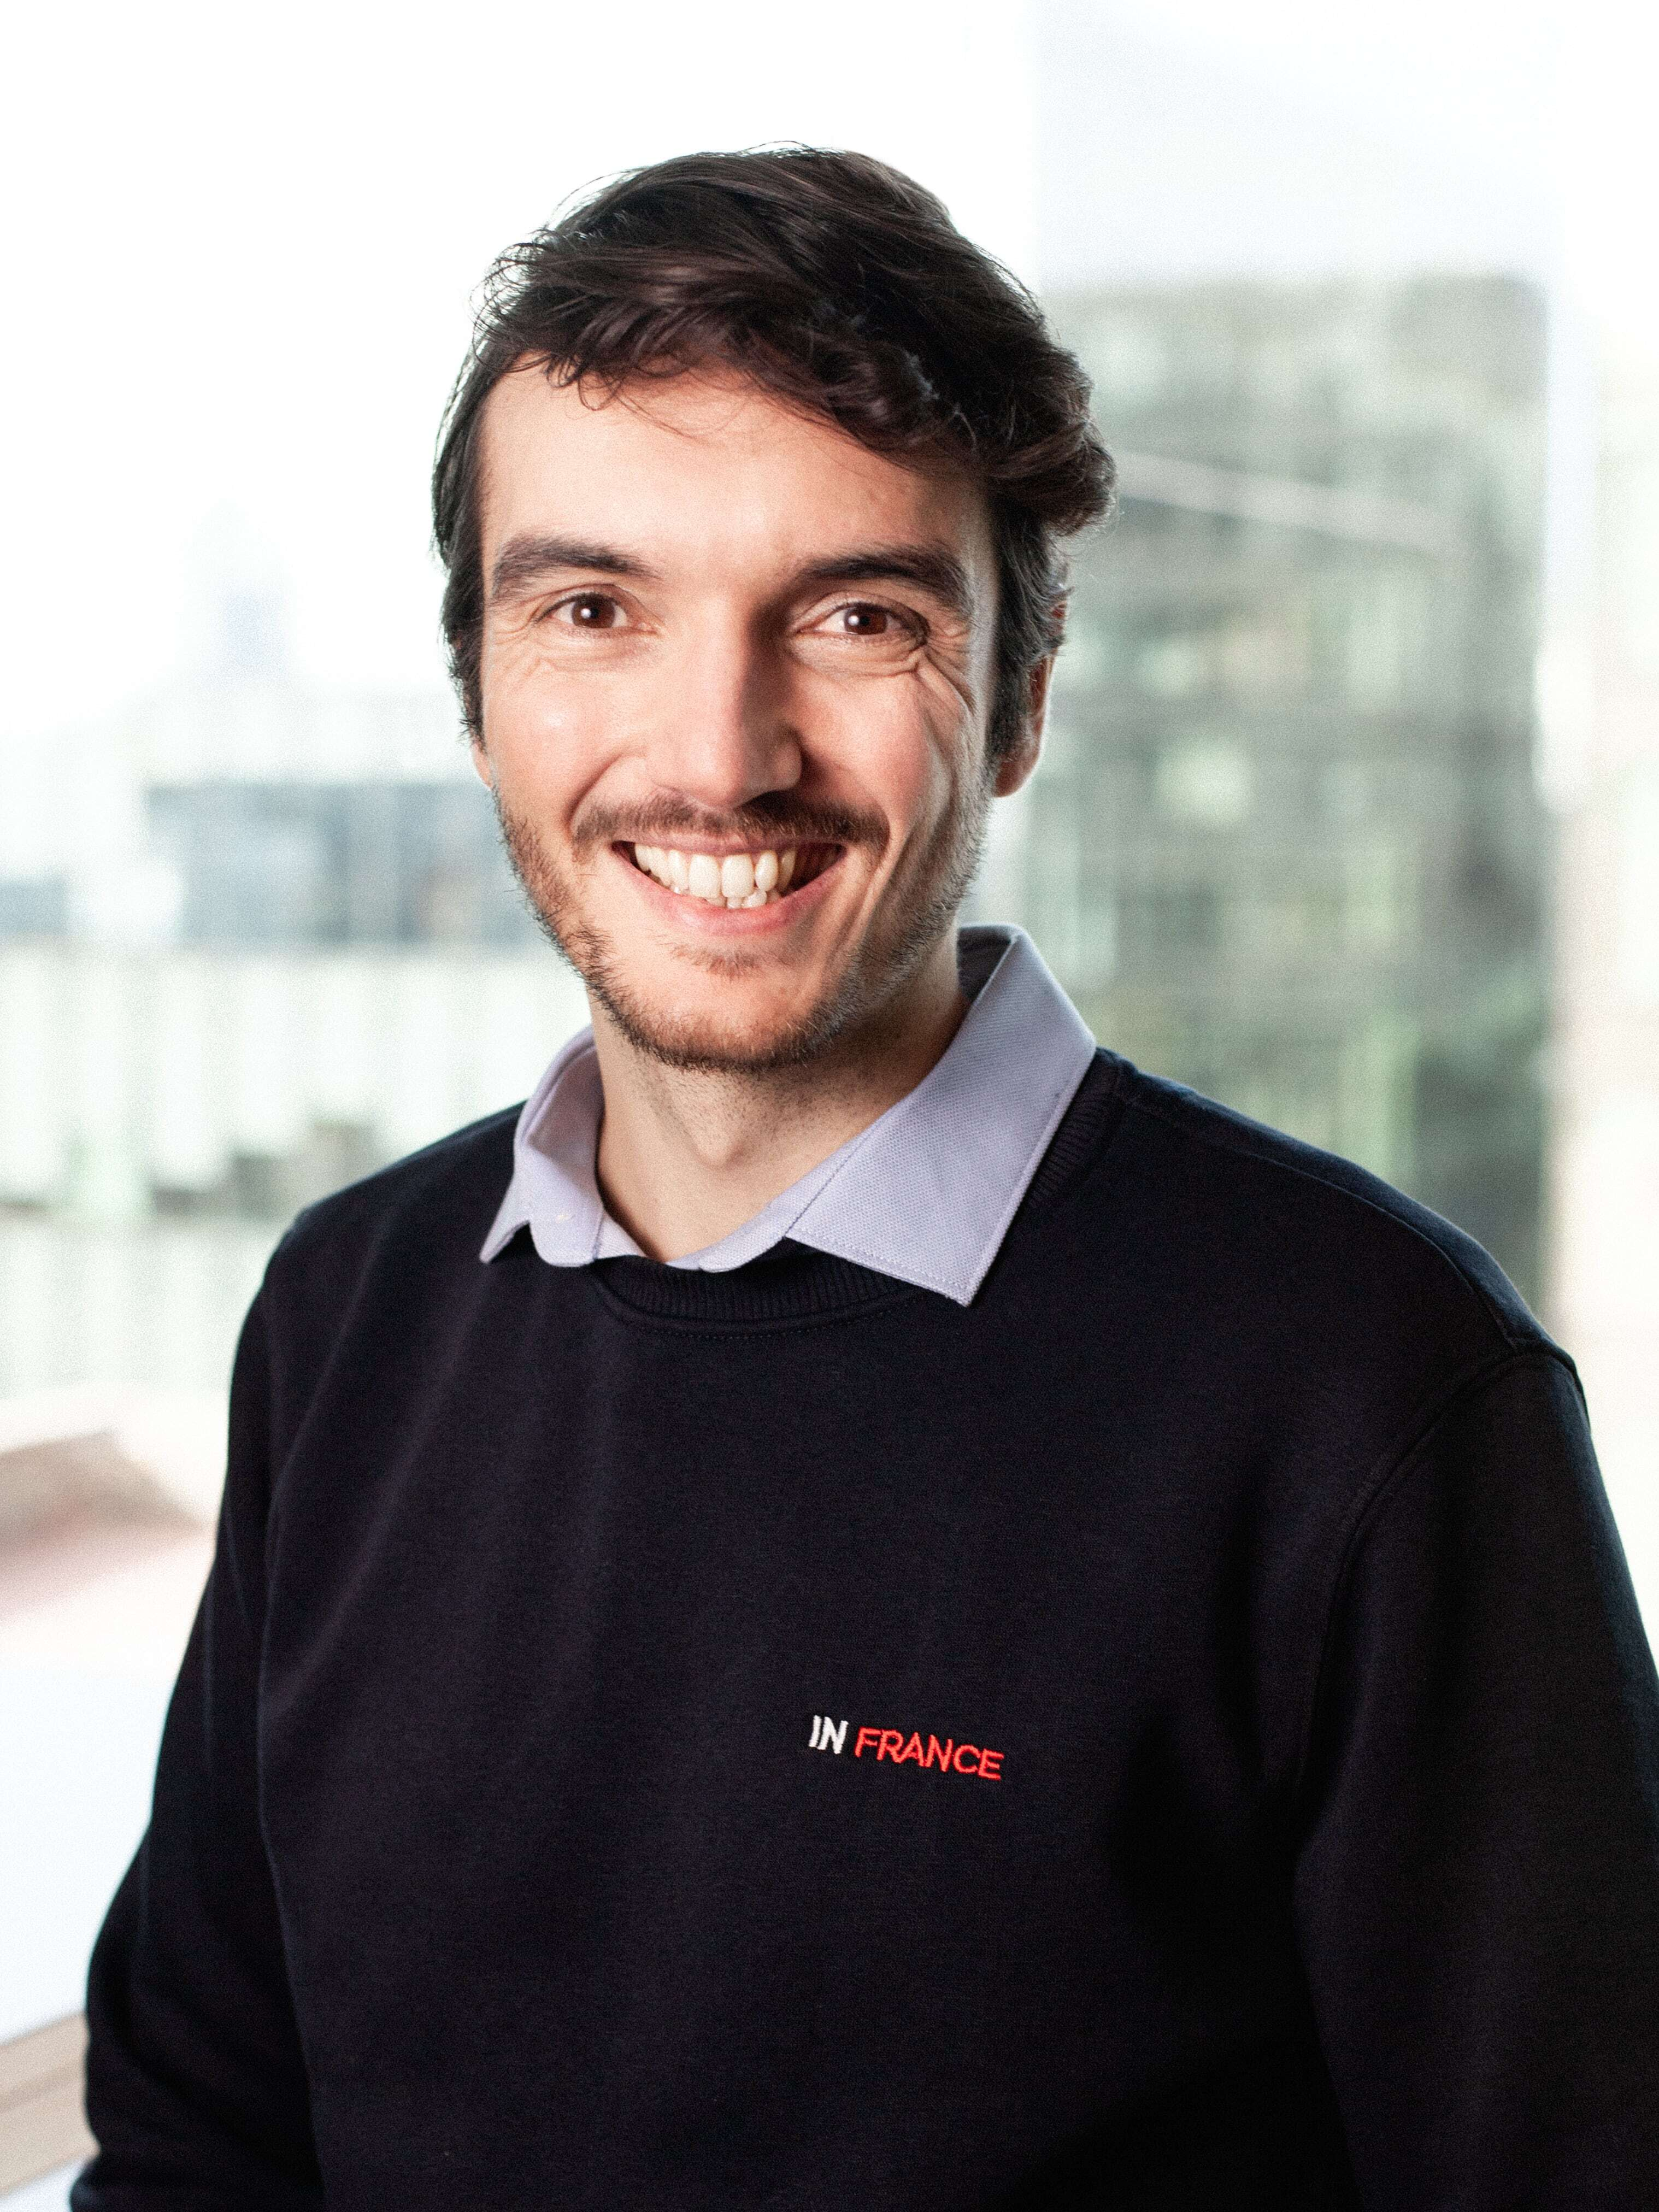
\includegraphics[width=5cm]{image/trombine-christophe}
        \end{columns}
    \end{frame}


    \section{Les origines}\label{sec:origines}
    \begin{frame}{Présentation de Python}{Qu'est-ce que Python~?}
        C'est une syntaxe, un langage de programmation et \textit{c'est tout}\footnote{Python is just an idiom, \url{https://github.com/phe-sto/Python-is-just-a-syntax}}~!
        \bigbreak
        C'est une syntaxe qui se veut facile à lire et à écrire, un langage de programmation qui se veut simple et complet.
        \bigbreak
        \begin{columns}
            \column{0.7\textwidth}
            Est-ce qu'il est rapide~? Ou lent~? Ni l'un ni l'autre, c'est un langage de programmation~!

            Sur quels systèmes d'exploitation s'exécute-t-il~? Sur aucun, c'est un langage de programmation, une syntaxe~!
            \bigbreak
            Une fois la syntaxe Python écrite, elle ne fait plus rien.
            Il faut un environnement d'exécution pour l'exécuter, comme un interpréteur Python.
            \column{0.3\textwidth}
            \centering
            
\includegraphics[width=4cm]{image/useless-python}
        \end{columns}
    \end{frame}

    \begin{frame}{Présentation de Python}{Comment exécuter le code Python~?}
        Une fois le programme écrit, il faut l'exécuter.

        Les environnements d'exécution possible sont innombrables~!
        Il en existe des plus spécifiques à une application comme \href{https://www.anaconda.com/}{Anaconda} pour le data science, ou à une plateforme comme \href{https://micropython.org/}{MicroPython}, sinon un plus généraliste comme l'interpréteur \href{https://github.com/python/cpython}{CPython}.
        \bigbreak
        Cette exécution peut résulter de~:
        \begin{itemize}
            \item Une interprétation d'un bytecode généré à la volée comme avec l'interpréteur \href{https://github.com/python/cpython}{CPython}.
            \item Une compilation d'un code Python, transpilé en C par \href{https://cython.org/}{Cython} et enfin compilé en binaire classique.
            \item Compilation directe dans l'environnement \href{https://micropython.org/}{MicroPython} vers une cible embarquée comme un MCU ARM~.
            \item Compilation à la volée dans une VM comme \href{https://pypy.org/}{PyPy} ou \href{https://www.graalvm.org/python/}{GraalVM} et son compilateur JIT.
        \end{itemize}
    \end{frame}

    \begin{frame}{Présentation de Python}{Comment exécuter le code Python~?}
        \begin{footnotesize}
            Liste non exhaustive des environnements d'exécution~:
            \begin{columns}
                \column{0.7\textwidth}
                \begin{itemize}
                    \item \href{https://github.com/python/cpython}{CPython}~: L'interpréteur de référence, écrit en C, il est le plus
                    \item \href{https://pypy.org/}{PyPy}~: Un interpréteur Python écrit en Python.
                    \item \href{https://cython.org/}{Cython}~: Un transpileur Python vers C, pour accélérer les parties critiques.
                    \item \href{https://www.graalvm.org/python/}{GraalVM}~: Un interpréteur Python sur une (J)VM polyglotte, avec un compilateur JIT.
                    \item \href{https://micropython.org/}{MicroPython}~: Python pour les microcontrôleurs.
                    \item \href{https://github.com/google/grumpy}{Grumpy}~: Un transpileur Python vers Go, qui a permis à Google/Youtube de migrer des millions de lignes de code Python vers Go.
                    \item \href{https://www.jython.org/}{Jython}~: Python sur la JVM, Java Virtual Machine.
                    \item \href{https://ironpython.net/}{IronPython}~: Python sur le CLR, Common Language Runtime de .NET.
                \end{itemize}
                \column{0.3\textwidth}
                \centering
                
\includegraphics[width=4cm]{image/python-logo}
            \end{columns}
        \end{footnotesize}
    \end{frame}

    \begin{frame}{Présentation de Python}{Les différents types d'exécution}
        \centering
        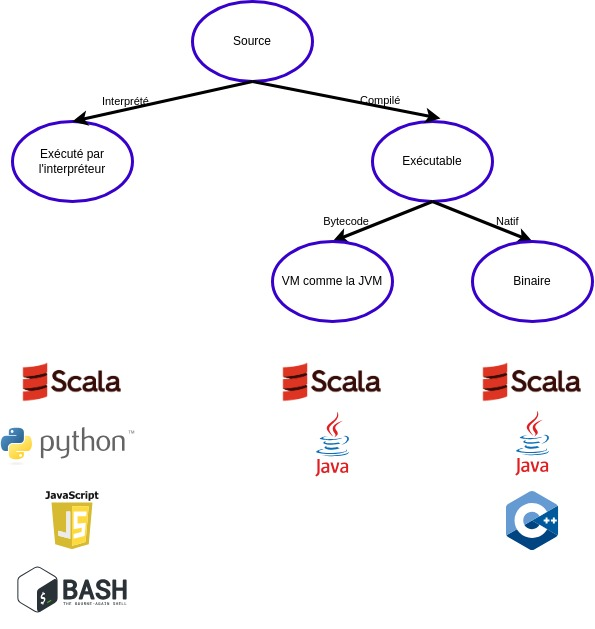
\includegraphics[width=7cm]{image/code-inter-vs-compiled}
    \end{frame}

    \begin{frame}{Présentation de Python}{L'interpréteur CPython domine\footnote{\label{python-usage}Python usage in 2021 and 2022, \url{https://lp.jetbrains.com/python-developers-survey-2022/}}}
        \centering
        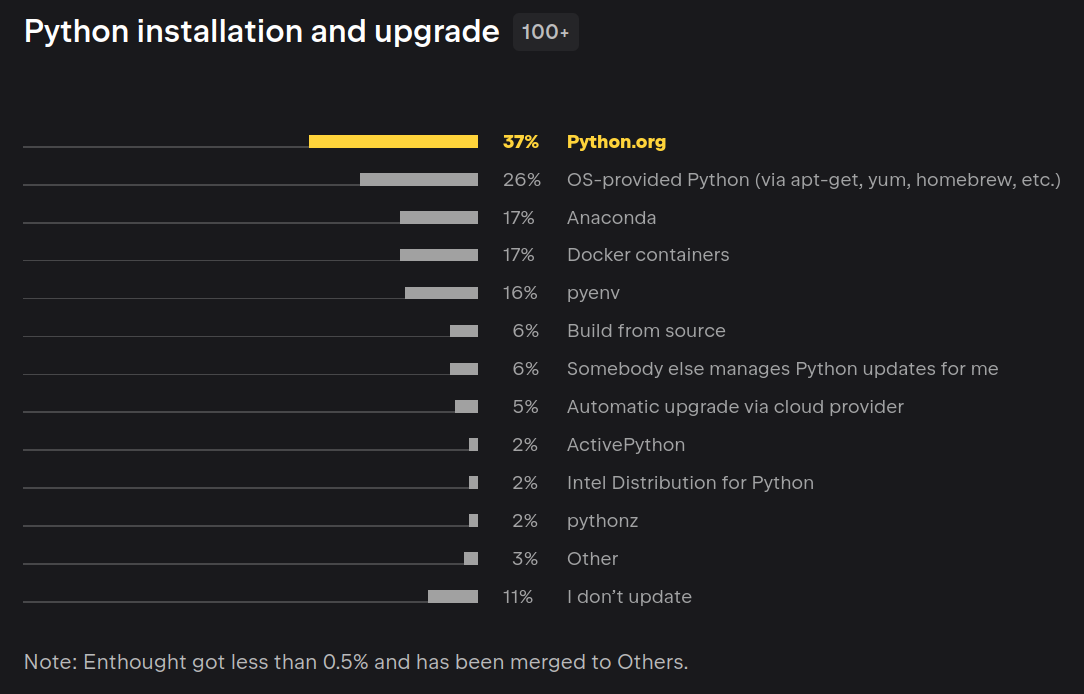
\includegraphics[width=10cm]{image/survey-install}
    \end{frame}

    \begin{frame}{Présentation de Python}{L'interpréteur CPython est open source}
        \begin{columns}
            \column{0.8\textwidth}
            Sous licence BSD, l'interpréteur CPython est open source.

            Elle permet d'utiliser cette technologie dans toutes les applications, même commerciales sans restriction.
            \bigbreak
            La majeure partie de l'écosystème est aussi OS.
            \column{0.2\textwidth}
            \centering
            
\includegraphics[width=2.5cm]{image/python-gift}
        \end{columns}
        \bigbreak
        \centering
        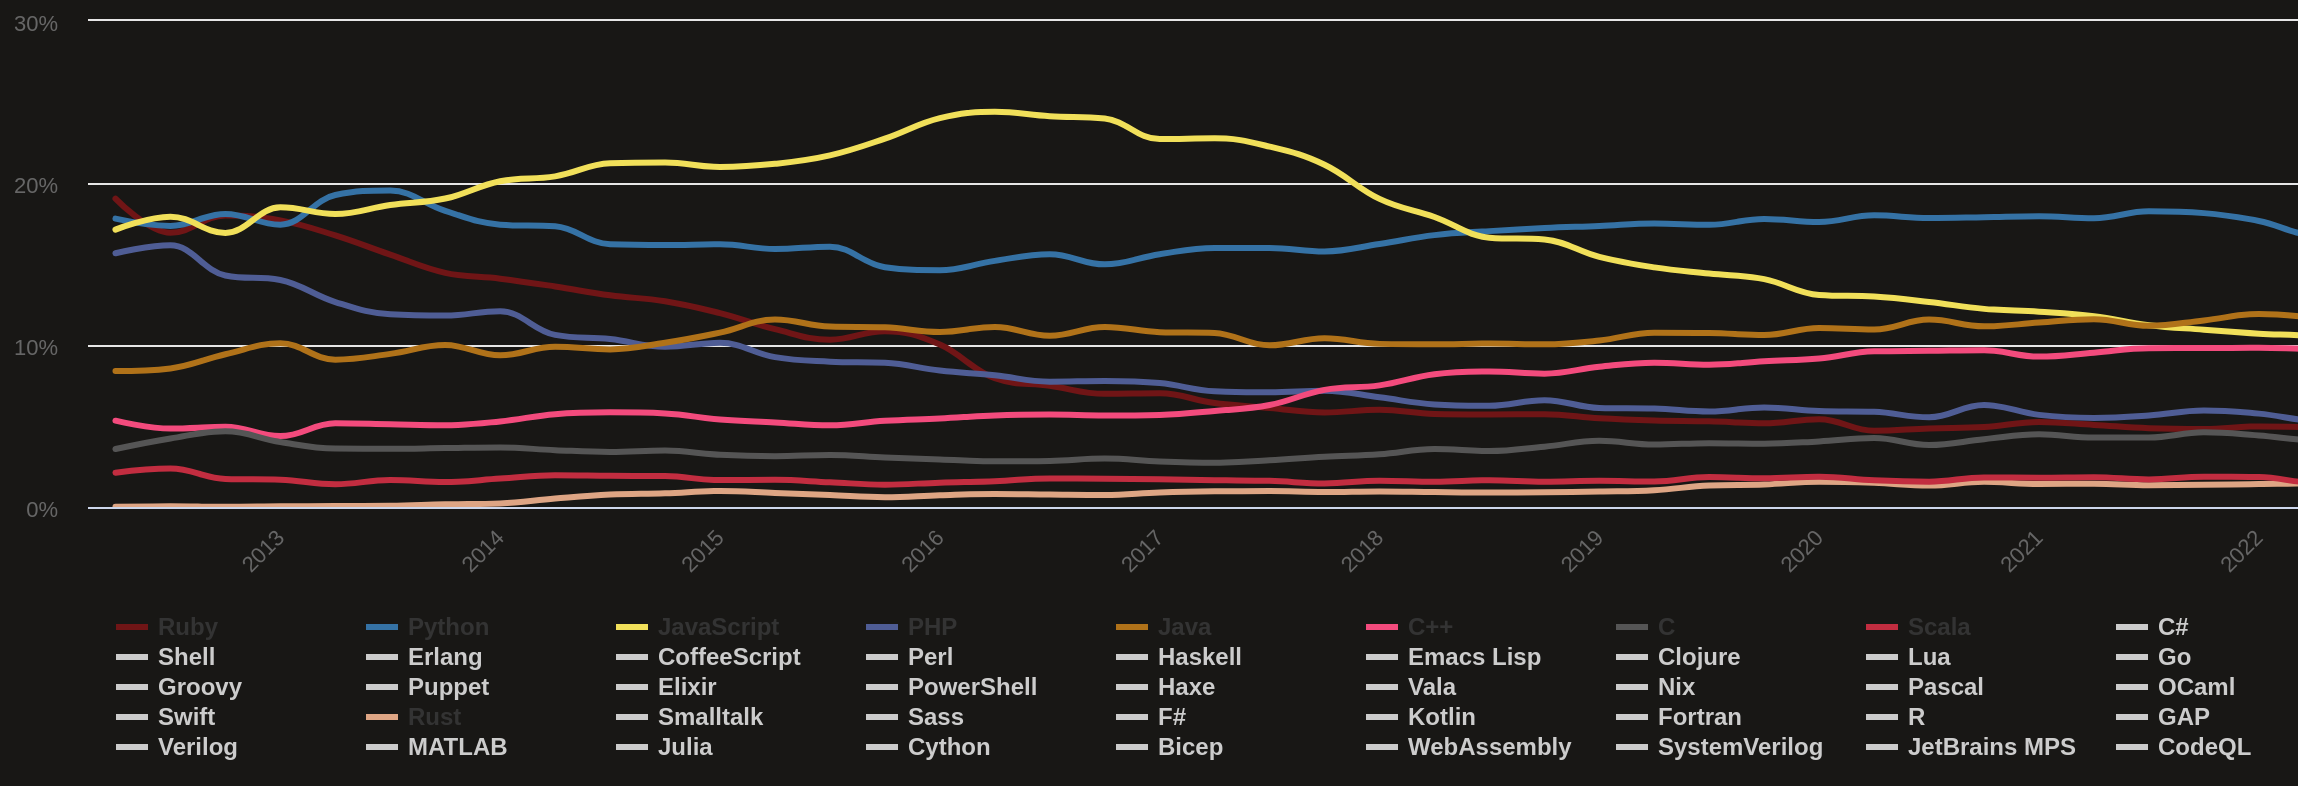
\includegraphics[width=9.5cm]{image/github-stats} \\ Statistiques GitHub \footnote{A small place to discover languages in GitHub, \url{https://madnight.github.io/githut/\#/pull_requests/2024/1}} \\
    \end{frame}

    \subsection{Les usages}\label{subsec:usages}

    \begin{frame}{Présentation de Python}{Les usages\cref{python-usage}}
        \centering
        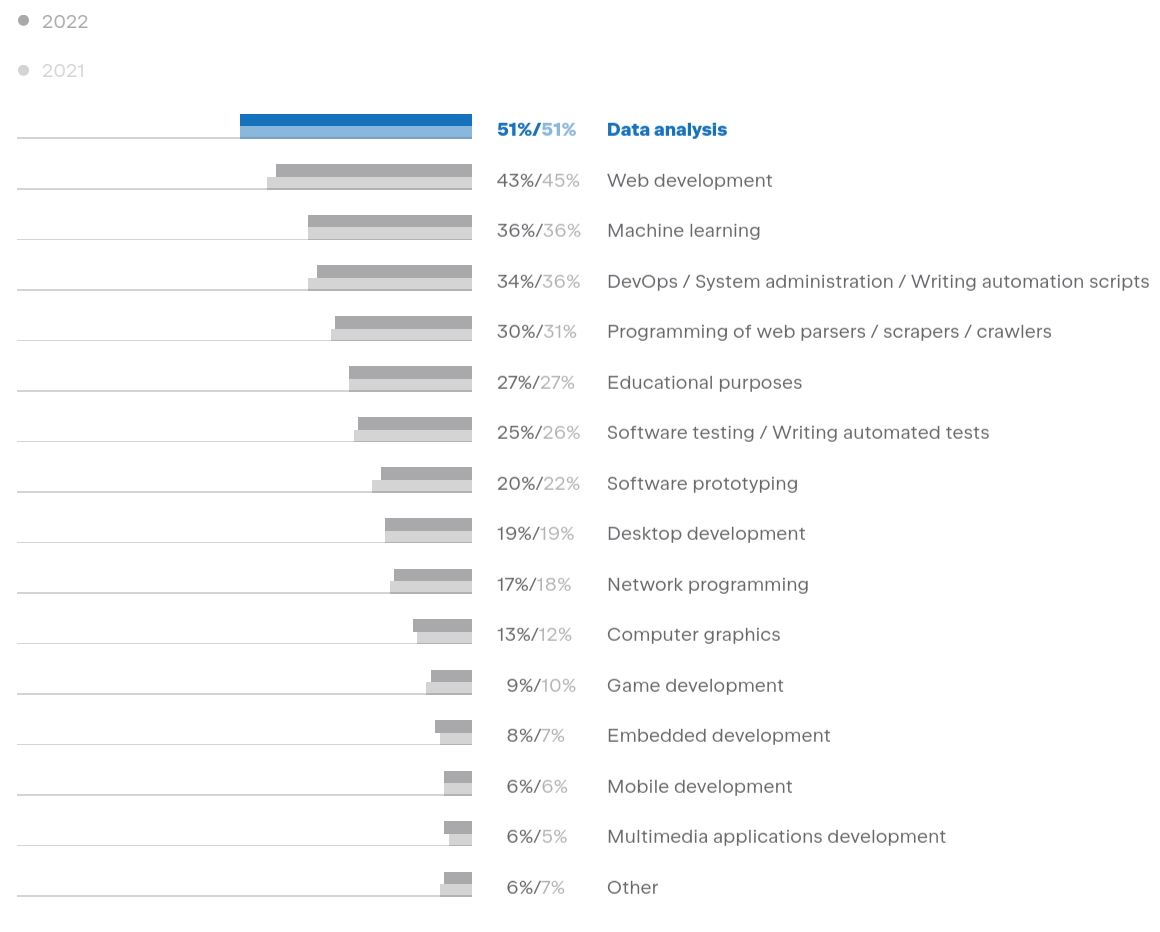
\includegraphics[width=9cm]{image/survey-usage}
    \end{frame}

    \subsection{Les dépendances}\label{subsec:dependances}

    \begin{frame}{Présentation de Python}{D'où viennent les dépendances~?\cref{python-usage}}
        \centering
        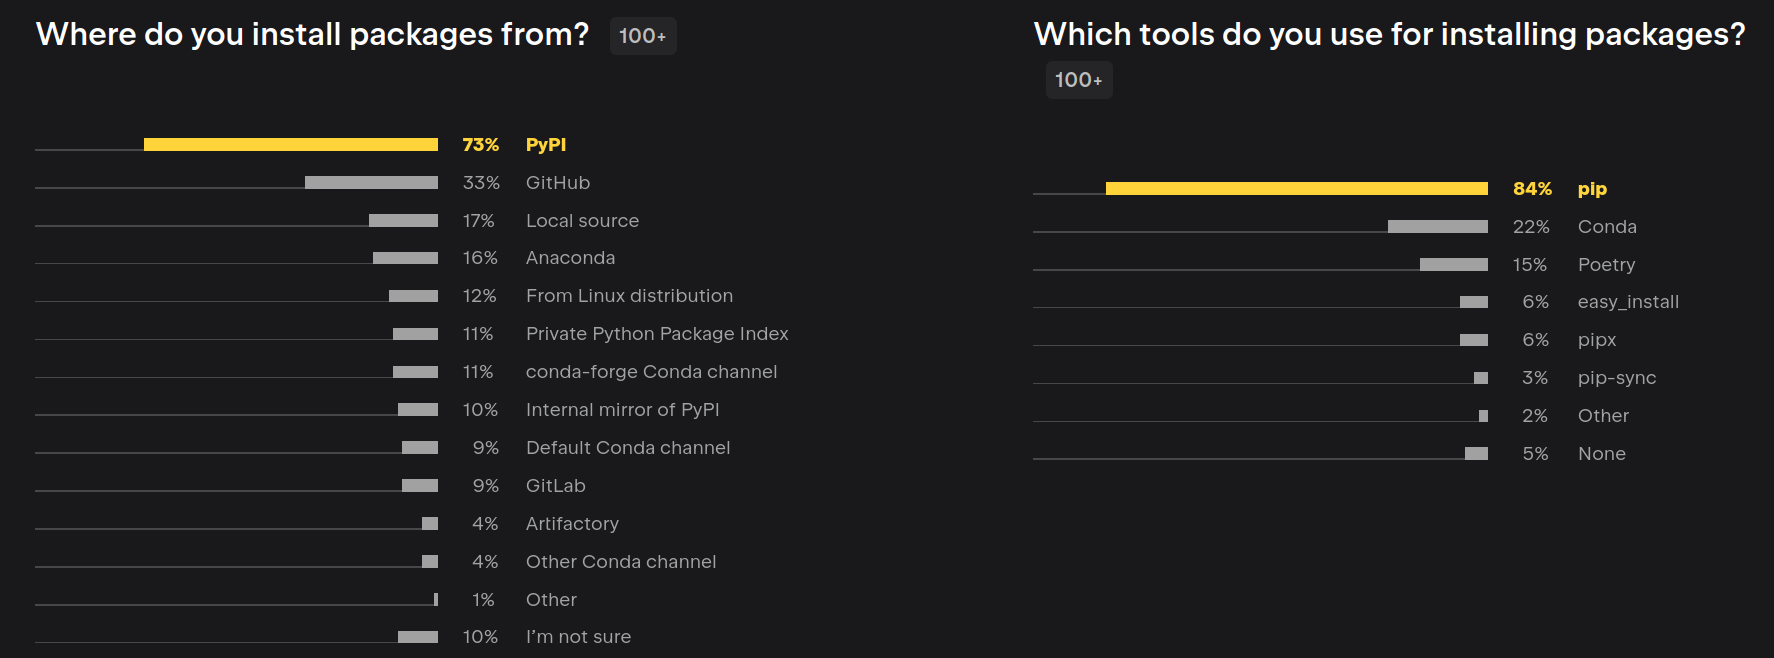
\includegraphics[width=12cm]{image/survey-packaging}
        \bigbreak
        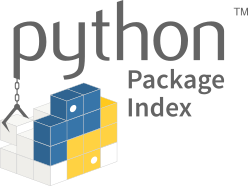
\includegraphics[width=3cm]{image/pypi-logo}
    \end{frame}


    \section{Historique}\label{sec:history}
    \begin{frame}{Historique}{Pourquoi créer un nouveau langage de programmation dans le années 90~?}
        \begin{footnotesize}
            \begin{columns}
                \column{0.5\textwidth}
                \centering
                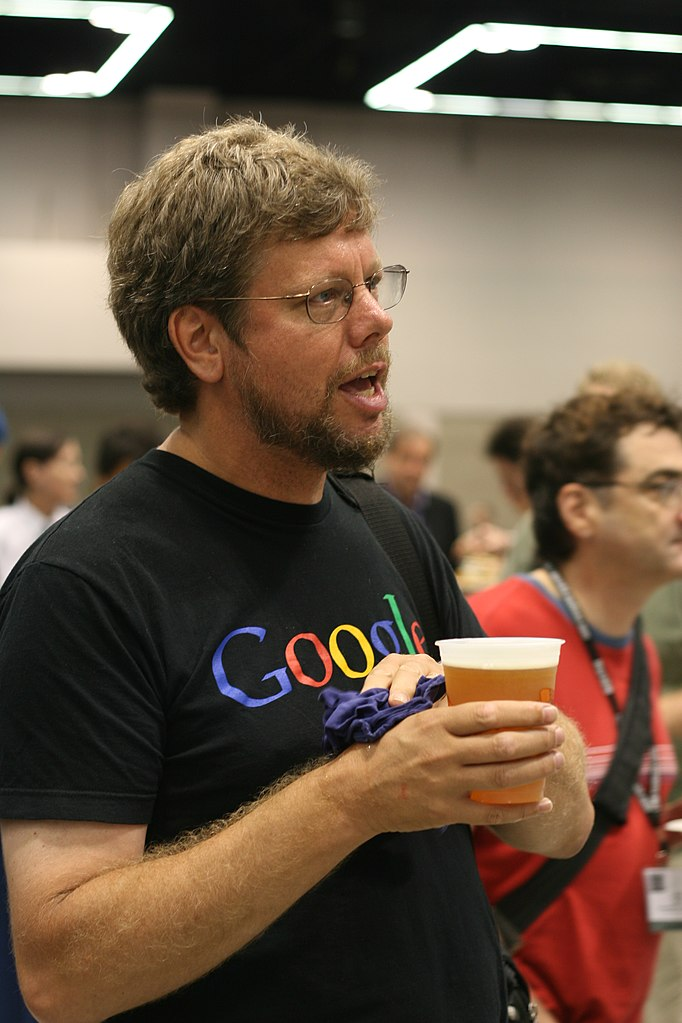
\includegraphics[width=2cm]{image/guido-van-rossum} \\ \href{https://www.flickr.com/photos/docsearls/}{Guido van Rossum (photo Doc Searls)} \\
                Le \textit{Benevolent Dictator For Life}, nomme son langage d'après le \textit{Monty Python’s Flying Circus}.
                \bigbreak
                \textquote{Python is a language that has been designed to be easy to read and write, and is thus remarkably straightforward compared to many other programming languages.}
                \column{0.5\textwidth}
                \centering
                
\includegraphics[width=5cm]{image/sun-java-logo}
                \flushleft
                Java en 1995, par Sun Microsystems, fait pour \textbf{vendre les PC et serveurs} de la marque.
                \bigbreak
                Son atout~: \textquote{Its syntax is similar to C and C++, but it omits many of the features that make C and C++ complex, confusing, and unsafe.}\footnotemark
            \end{columns}
        \end{footnotesize}
        \footnotetext{Oracle, Java Virtual Machine Specification, \url{https://docs.oracle.com/javase/specs/jvms/se8/html/jvms-1.html}}
    \end{frame}


    \section{PEP et les bonnes pratiques}\label{sec:pep-good-pratices}

    \begin{frame}{Bonnes pratiques, l'approche de Python}
        \begin{itemize}
            \item Python a une syntaxe éloignée des langages de son temps qui sont toutes déclinées de celle du C. Les syntaxes de C, C++, C\#, Java et même JavaScript
            \item Le pari d'une nouvelle syntaxe était risqué, mais G. Van Rossum souhaite une meilleure lisibilité
            \item \textquote{code is read much more often than it is written. The guidelines provided here are intended to improve the readability of code and make it consistent across the wide spectrum of Python code. As PEP 20 says, \textbf{Readability counts}}\footnote{Guido Van Rossum, \url{https://peps.python.org/pep-0008/}}
        \end{itemize}
    \end{frame}

    \begin{frame}[fragile]
        \transdissolve
        \frametitle{Bonnes pratiques, l'approche de Python}
        \begin{lstlisting}
In [1]: import this
The Zen of Python, by Tim Peters

Beautiful is better than ugly.
Explicit is better than implicit.
Simple is better than complex.
Complex is better than complicated.
Flat is better than nested.
Sparse is better than dense.
Readability counts.
Special cases aren't special enough to break the rules.
Although practicality beats purity.
Errors should never pass silently.
Unless explicitly silenced.
In the face of ambiguity, refuse the temptation to guess.
There should be one-- and preferably only one --obvious way to do it.
Although that way may not be obvious at first unless you're Dutch.
Now is better than never.
Although never is often better than *right* now.
If the implementation is hard to explain, it's a bad idea.
If the implementation is easy to explain, it may be a good idea.
Namespaces are one honking great idea -- let's do more of those!
        \end{lstlisting}
    \end{frame}

    \begin{frame}[fragile]
        \transdissolve
        \frametitle{Bonnes pratiques, l'approche de Python}
        En cas d'oubli, le mantra de Python A.K.A The Zen of Python, est dans l'interpréteur~!

        \bigbreak

        Le bon sens paysan fait consensus dans tous les langages de programmation~!

    \end{frame}

    \begin{frame}[fragile]
        \transdissolve
        \frametitle{Bonnes pratiques, Python et PEP}
        \begin{columns}
            \column{0.5\textwidth}
            \begin{itemize}
                \item PEP est la convention de codage recommandée par Python, comme PEP8, le Style Guide for Python Code, à lire SVP
                \item Défini les espaces utiles à la lisibilité et les inutiles
                \item Snake\_case pour les variables
                \item Défini les casses et la déclaration~:
                \begin{itemize}
                    \item Attribut et méthode privé/publique~:
                \end{itemize}
            \end{itemize}
            \column{0.5\textwidth}
            \begin{lstlisting}[language=python]
class Case:
    public = 0

Case.public

Out[3]: 0

class Case:
    __private = 0

In [13]: Case.__private
---------------------------------------------------------------------------
AttributeError                            Traceback (most recent call last)
Cell In [13], line 1
----> 1 Case.__private

AttributeError: type object 'Case' has no attribute '__private'
            \end{lstlisting}
        \end{columns}
    \end{frame}

    \begin{frame}[fragile]
        \transdissolve
        \frametitle{Bonnes pratiques, Python et PEP}
        \begin{itemize}
            \item Déclaration des constantes en upper case avec underscore, comme la plupart des langages~:
            \begin{lstlisting}[language=python]
In [17]: PLANCK_CONSTANT = 6.62607015*(10^-34) # Upper case with underscore for constants

In [18]: PLANCK_CONSTANT = 42 # But constant those not really exists in Python

In [19]: PLANCK_CONSTANT
Out[19]: 42
            \end{lstlisting}
            \item Déclaration des classes en CamelCase et fonctions en snake\_case~:
            \begin{lstlisting}[language=python]
In [20]: class UnNomEnCamelCase:
...:     pass
...:

In [21]: def un_verbe_au_moins_en_snake_case():
...:     pass
...:
            \end{lstlisting}
        \end{itemize}

    \end{frame}

    \begin{frame}[fragile]{Bonnes pratiques, Python et PEP}
        \begin{itemize}
            \item Les commentaires, en ligne si possible~:
            \begin{lstlisting}[language=python]
In [22]: is_even = lambda x: x % 2 == 0  # Il est clair que l'on commente cette ligne mais c'est long

In [23]: # Retourne True pour un chiffre pair

In [24]: is_even = lambda x: x % 2 == 0
            \end{lstlisting}
            \item Favoriser l'indentation même si la syntaxe en ligne est valide, après les \textquote{:} des conditions et des déclarations~:
            \begin{lstlisting}[language=python]
def is_even(x):return x % 2 == 0 # Pas biennnn

def is_even(x):
    return x % 2 == 0 # Biennnn
            \end{lstlisting}
        \end{itemize}
    \end{frame}

    \begin{frame}[fragile]{Bonnes pratiques, Python et PEP}{Les modules}
        Un module est un fichier de code source contenant des déclarations et des définitions Python. Le nom du fichier est le nom du module avec l'extension \lstinline{.py} ajoutée.
        \bigbreak
        Les modules doivent avoir des noms courts, entièrement en minuscules. Les underscores peuvent être utilisés dans le nom du module si cela améliore la lisibilité.
        Les packages Python doivent également avoir des noms courts et entièrement en minuscules, bien que l’utilisation des underscores soit déconseillée\footnote{PEP 8 – Style Guide for Python Code, \url{https://peps.python.org/pep-0008/\#package-and-module-names}}.
        \bigbreak
        Par exemple~:
        \begin{lstlisting}[language=Bash]
$ ll
total 8
-rw-r--r-- 1 christophe christophe  0 mai   17 09:00 __init__.py
-rw-r--r-- 1 christophe christophe  0 mai   17 09:00 compute_price.py
-rw-r--r-- 1 christophe christophe  0 mai   17 09:00 server.py
        \end{lstlisting}
    \end{frame}

    \begin{frame}{Bonnes pratiques, l'IDE, une aide précieuse}
        \begin{columns}
            \column{0.5\textwidth}
            \begin{center}
                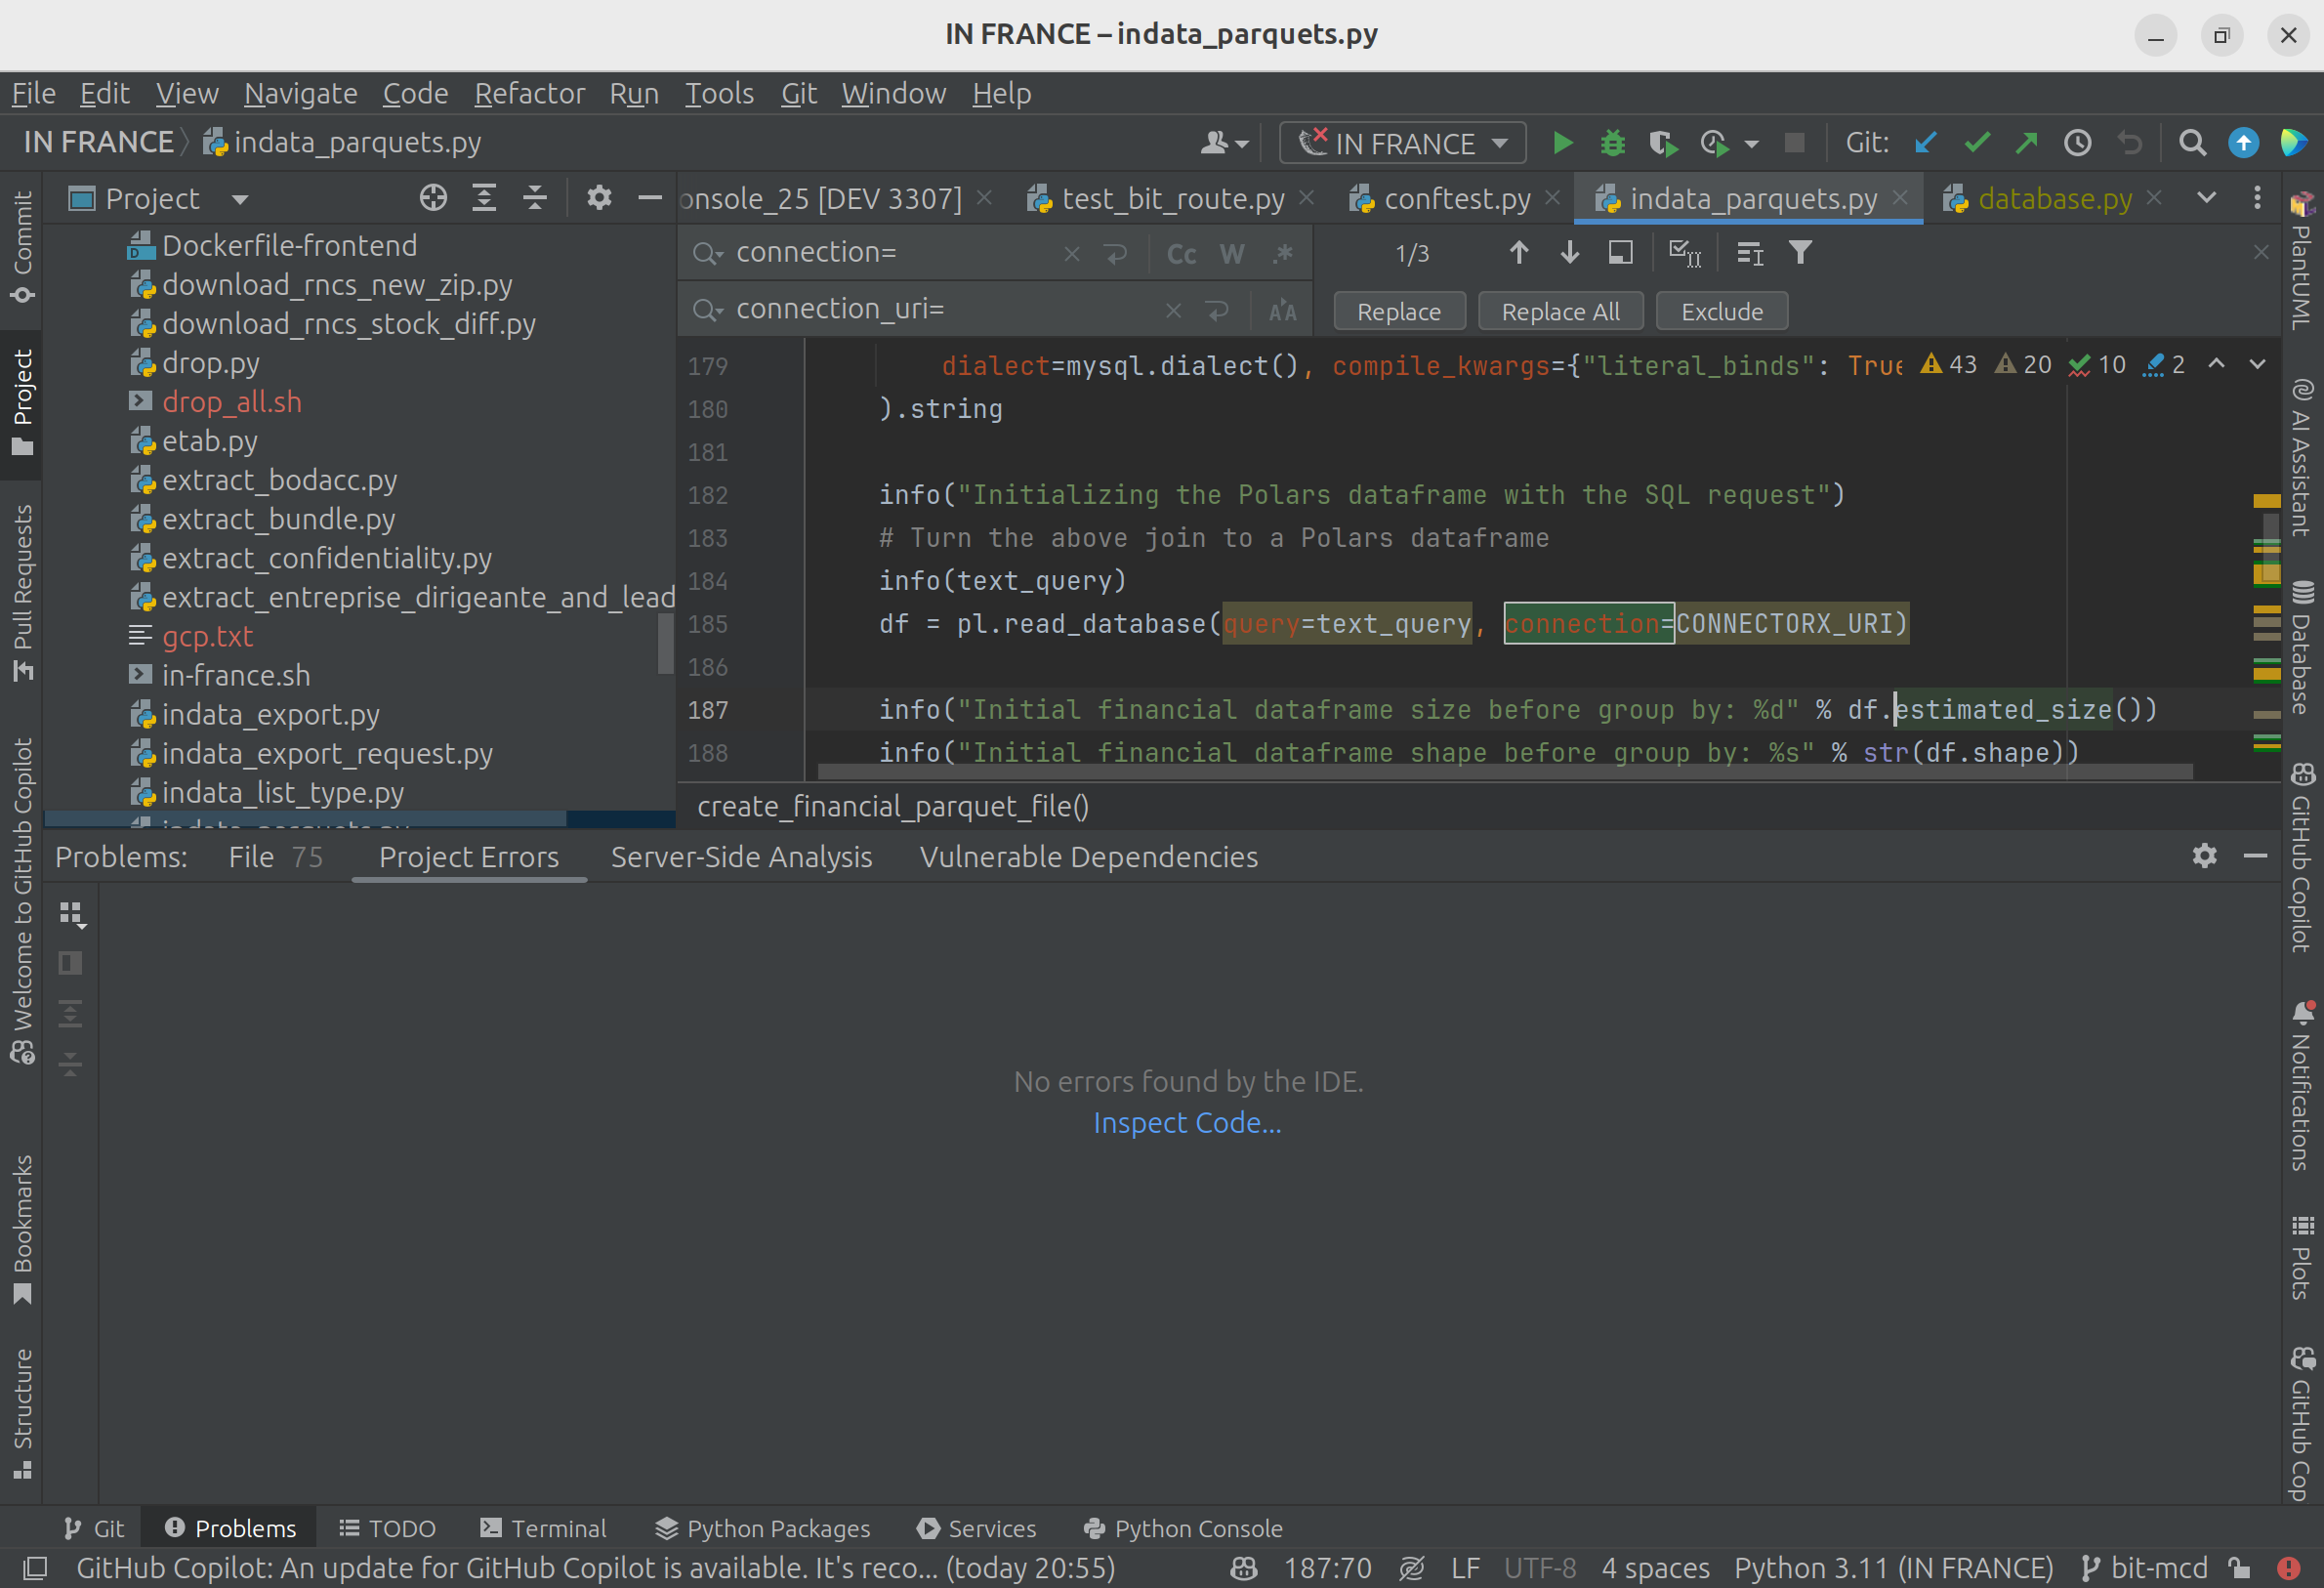
\includegraphics[width=5cm]{image/Pycharm-before-analysis}
            \end{center}
            \column{0.5\textwidth}
            \begin{center}
                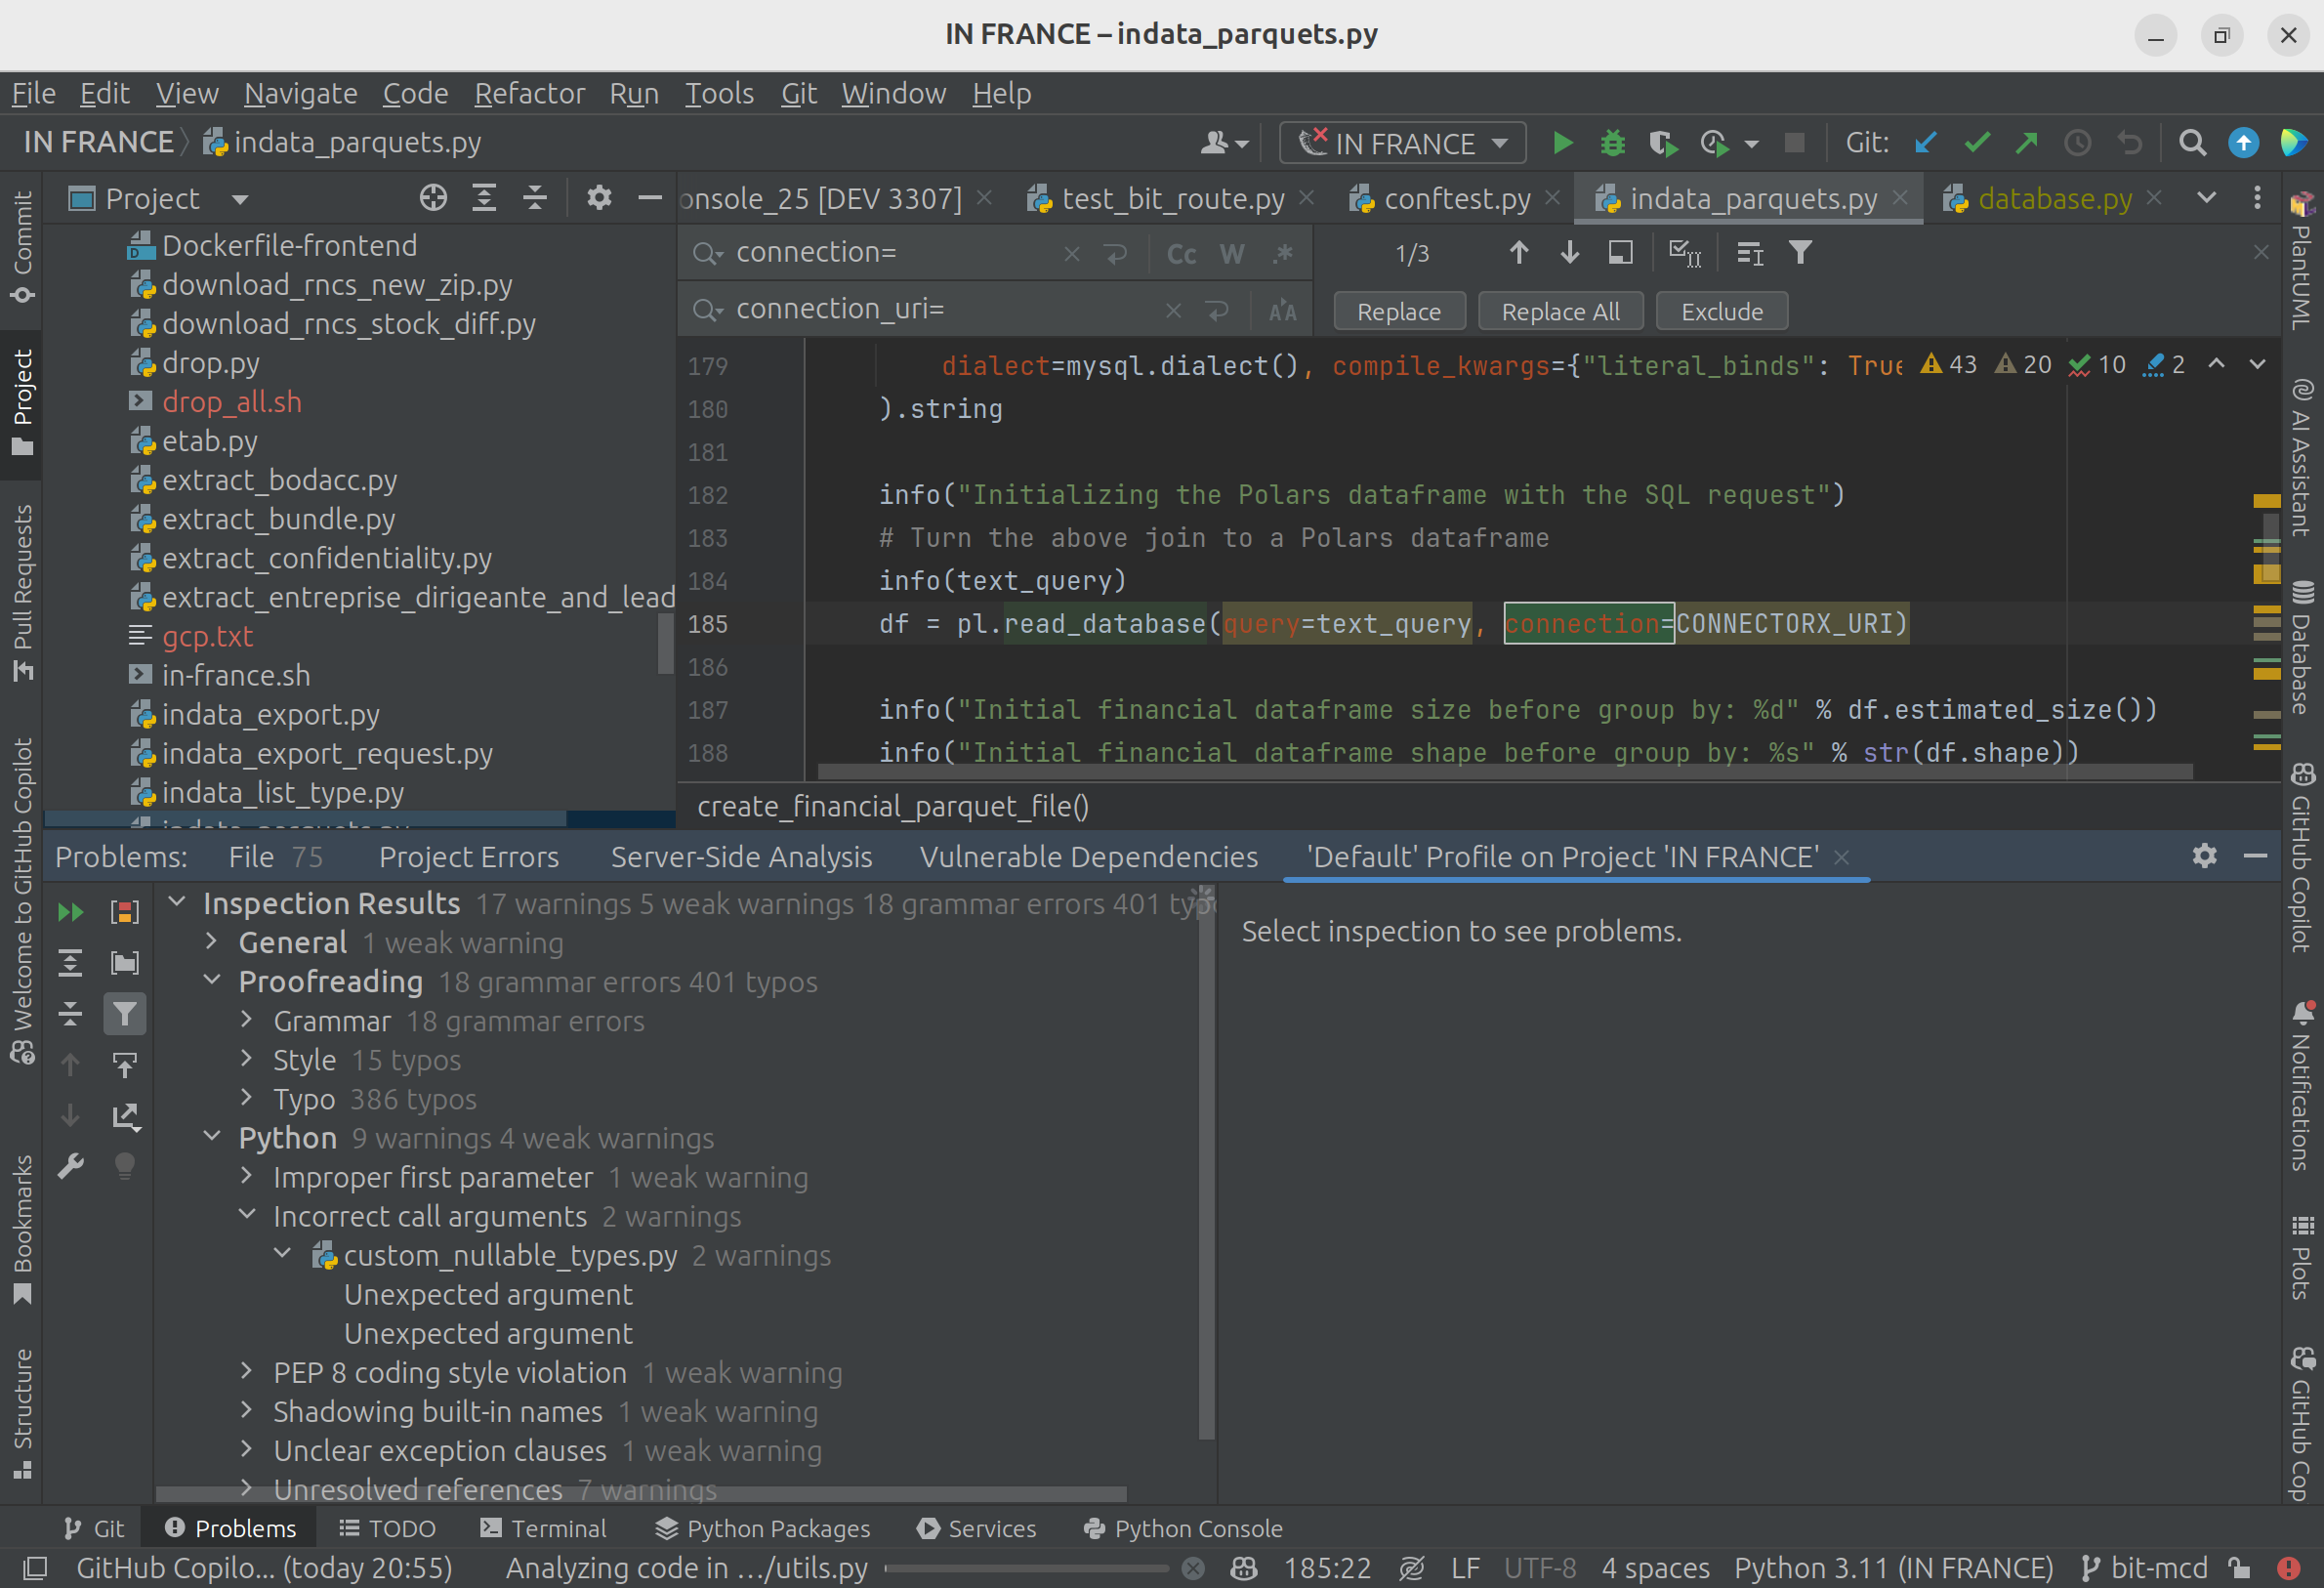
\includegraphics[width=5cm]{image/Pycharm-after-analysis}
            \end{center}
        \end{columns}
        \bigbreak

        \begin{flushleft}
            Dans la fenêtre dédiée aux divers warnings et erreurs, après analyse du project, les IDEs modernes détaillent de multiples types d'erreurs et warnings.
            Ils peuvent même les corriger automatiquement.

            Une liste non exhaustive des IDEs ouverts~:
            \begin{itemize}
                \item VS Code (Avec Black formatter et Pylint)
                \item Pycharm pour Python
                \item Zed (\url{https://zed.dev/}, sur Mac OS et Linux pour l'instant uniquement)
            \end{itemize}
        \end{flushleft}

    \end{frame}

    \begin{frame}{Bonnes pratiques, l'IDE, intégration à des outils tiers}

        \centering
        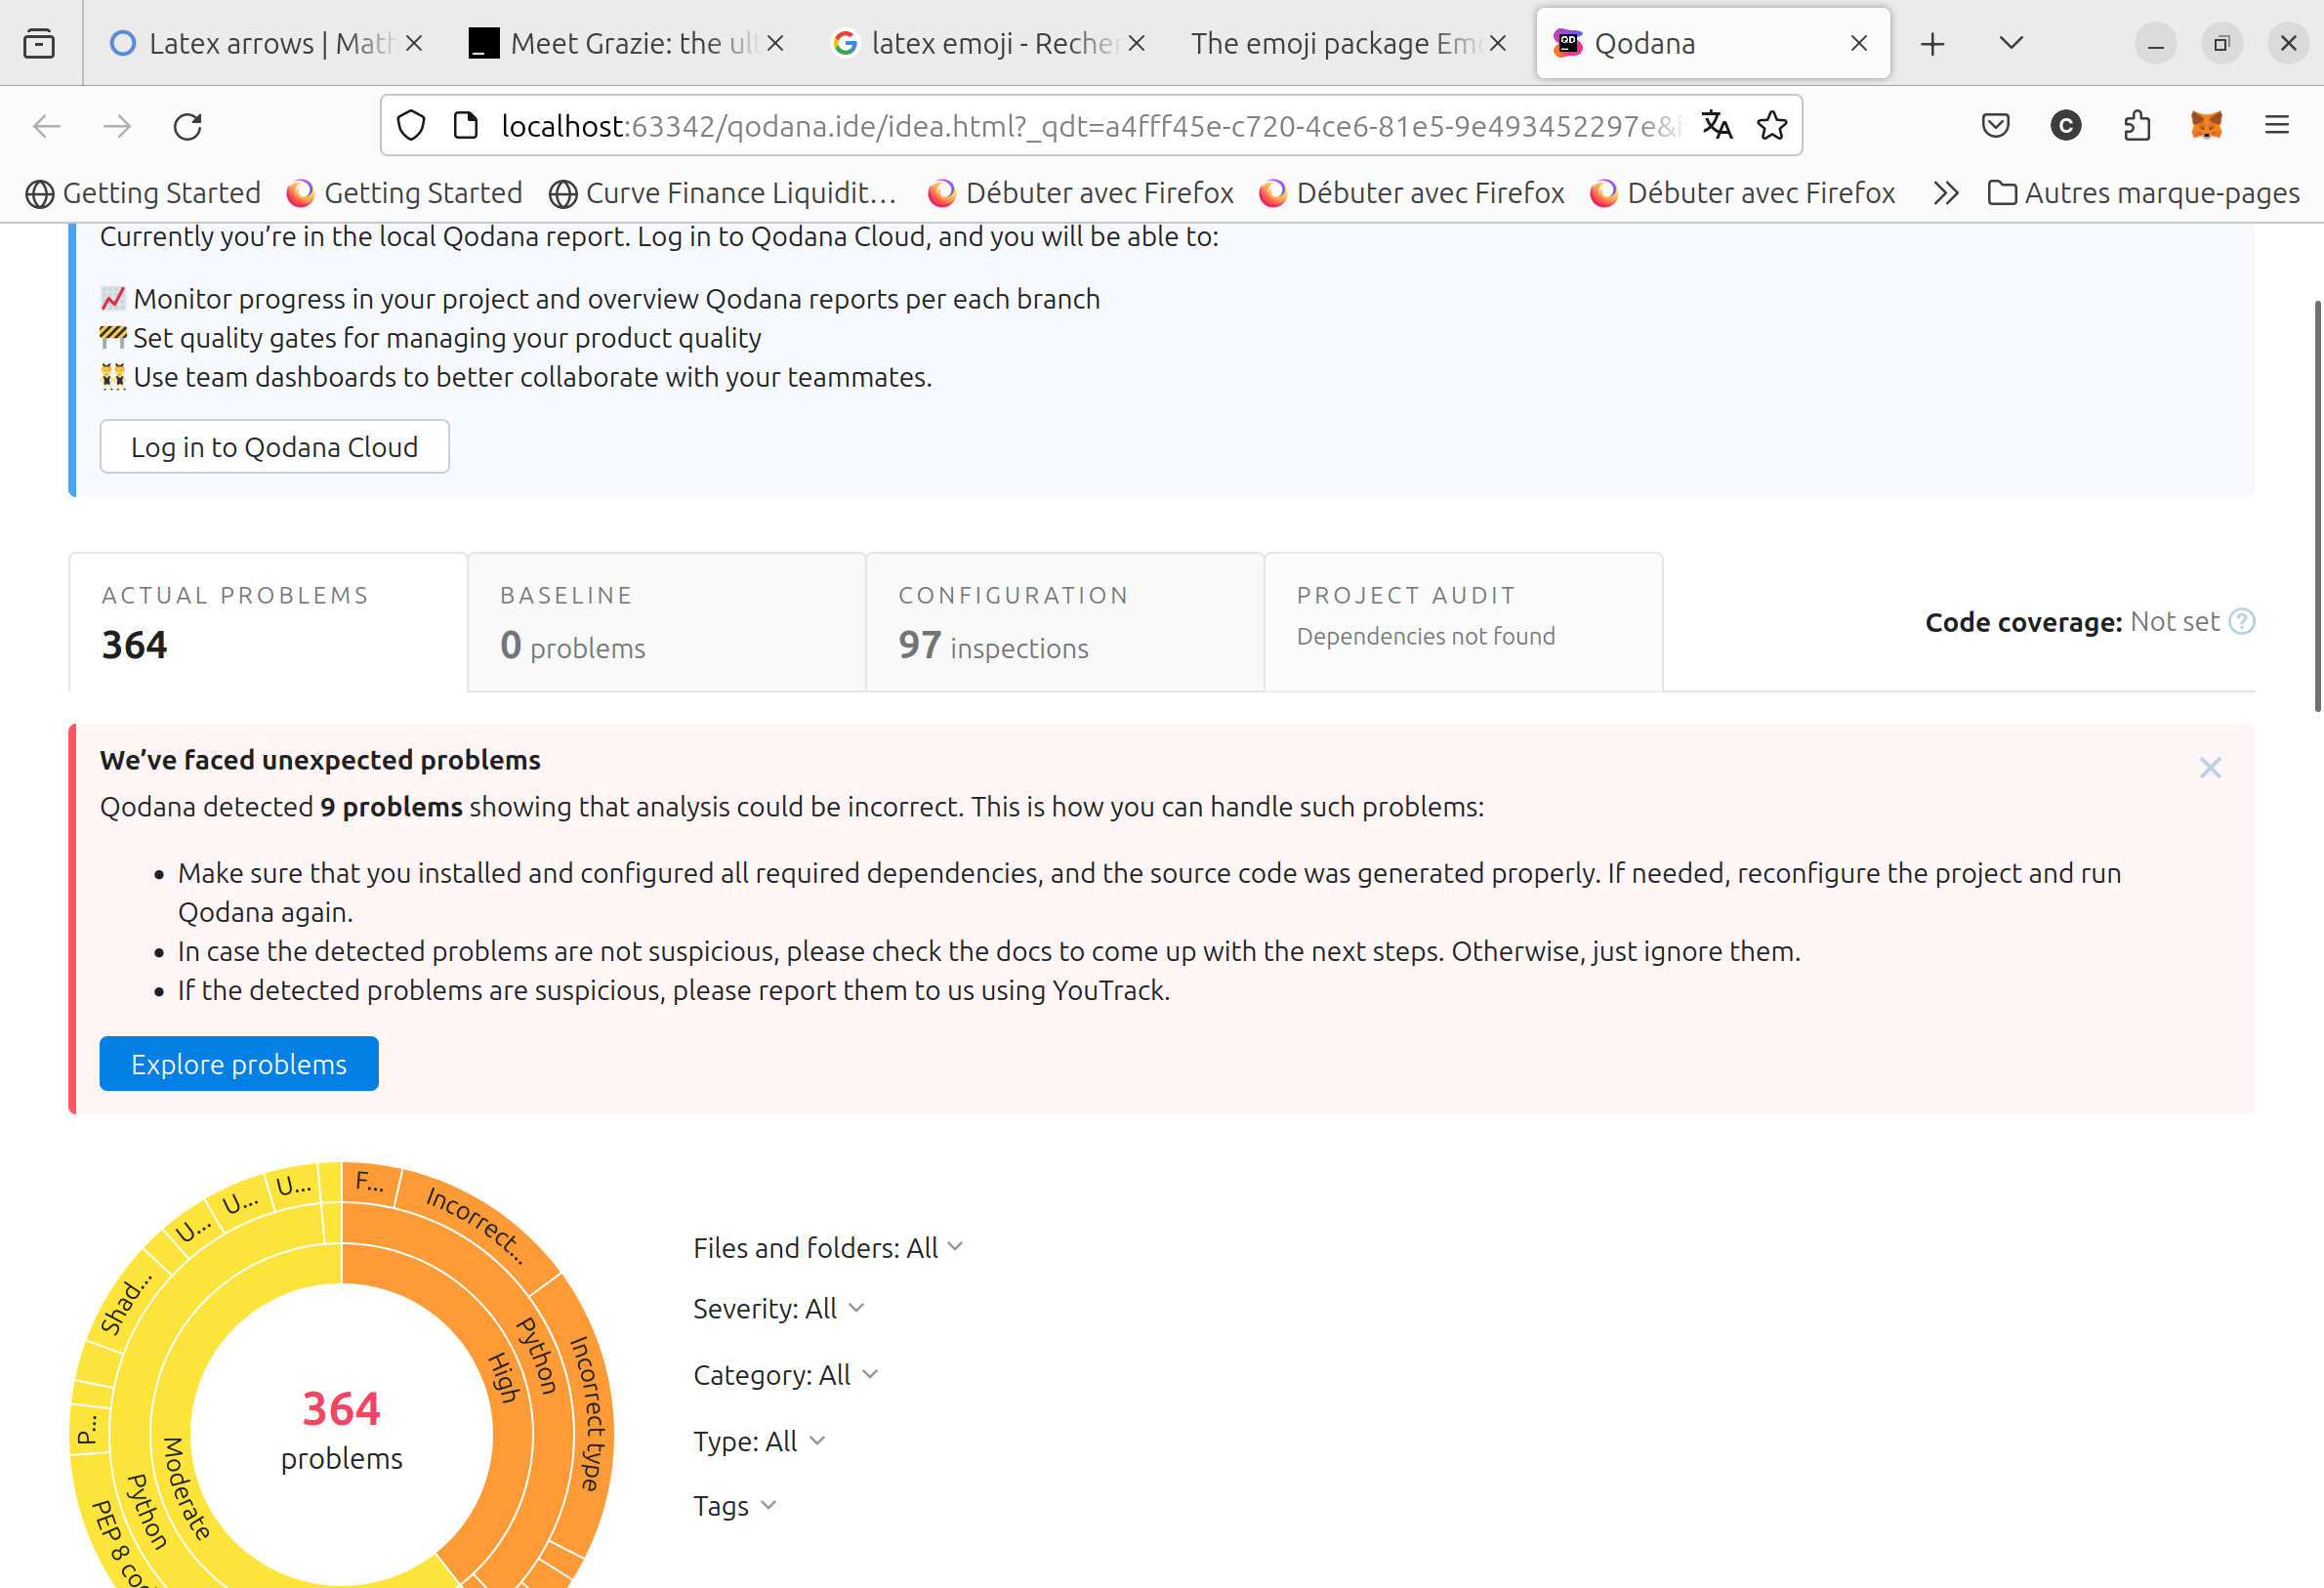
\includegraphics[width=5cm]{image/Qodana-result}

        \bigbreak

        \begin{flushleft}
            Certains plugins peuvent se connecter à des applications dédiées à l'analyse des sources comme SonarQube \emoji{flag-switzerland}, Qodana, etc.
            Ils permettent une analyse plus complète et d'enregistrer des indicateurs permettant de suivre l'évolution dans le temps de la qualité des sources du projet.
        \end{flushleft}
    \end{frame}

    \begin{frame}{Bonnes pratiques, l'IDE, lire les indications}

        \begin{itemize}
            \item VS Code ou Pycharm ont toutes ces fonctionnalités modernes
            \item Dans la carte, sur le côté on voit rapidement les soucis sur tout un fichier
            \bigbreak
            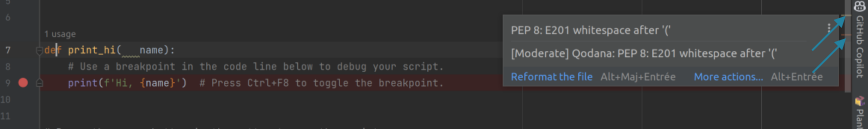
\includegraphics[width=8cm]{image/Pycharm-minimap}
            \item Dans le code source en cours d'édition
            \bigbreak
            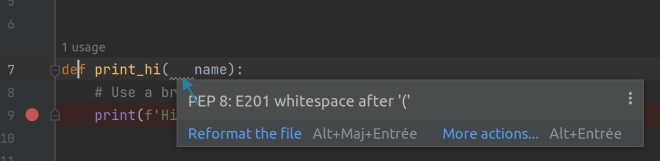
\includegraphics[width=8cm]{image/Pycharm-waring-in-code}
        \end{itemize}

    \end{frame}


    \section{Où développer?}\label{sec:where}


    \begin{frame}{Les environnements de développement}
        \begin{small}
            Il existe de nombreuses possibilités pour développer en Python.
            Dans des environnements plus ou moins lourds, plus ou moin complexes.
            \begin{itemize}
                \item IDLE, \textit{Integrated DeveLopment Environment} l'IDE de base de Python, simpliste et lui-même codé en Python.
                Il contient quand même un débuggeur~!
                \item IPython, un Shell Python évolué avec autocompletion.
                Aussi appellé REPL \textit{Read-Evaluate-Print Loop}, il est utile pour tester un petit nombre de lignes.
                \item Jupyter, un notebook Python, très utilisé en data science.
                Il permet de mettre en forme son développement avec du markdown pour une présentation claire et une documentation intégrée.
                Pas de débuggeur \emoji{exploding-head}.
                \item VS Code, un éditeur de code à compléter avec des plugins, a un débuggeur, un analyseur de code, un formateur de code, etc.
                \item PyCharm, un IDE complet dédié au Python, avec un débuggeur, un analyseur de code, un formateur de code, etc.
                Il est celui conseillé sur \url{python.org} dans la brochure\footnote{PSF Python Brochure Vol. I final Download .pdf, \url{https://brochure.getpython.info/media/releases/psf-python-brochure-vol.-i-final-download.pdf/view}} (à lire).
            \end{itemize}
        \end{small}
    \end{frame}

    \begin{frame}{Les environnements de développement}{Les plus populaires\cref{python-usage}}
        \centering
        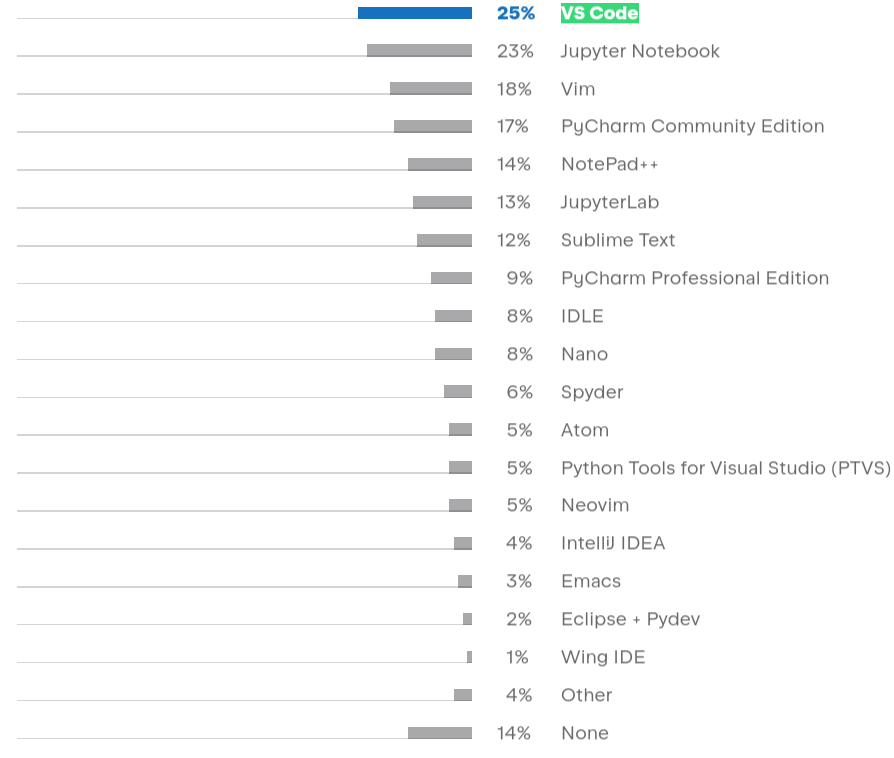
\includegraphics[width=9cm]{image/survey-ides}
    \end{frame}

    \begin{frame}{Les environnements de développement}{Le REPL IPython}
        \begin{center}
            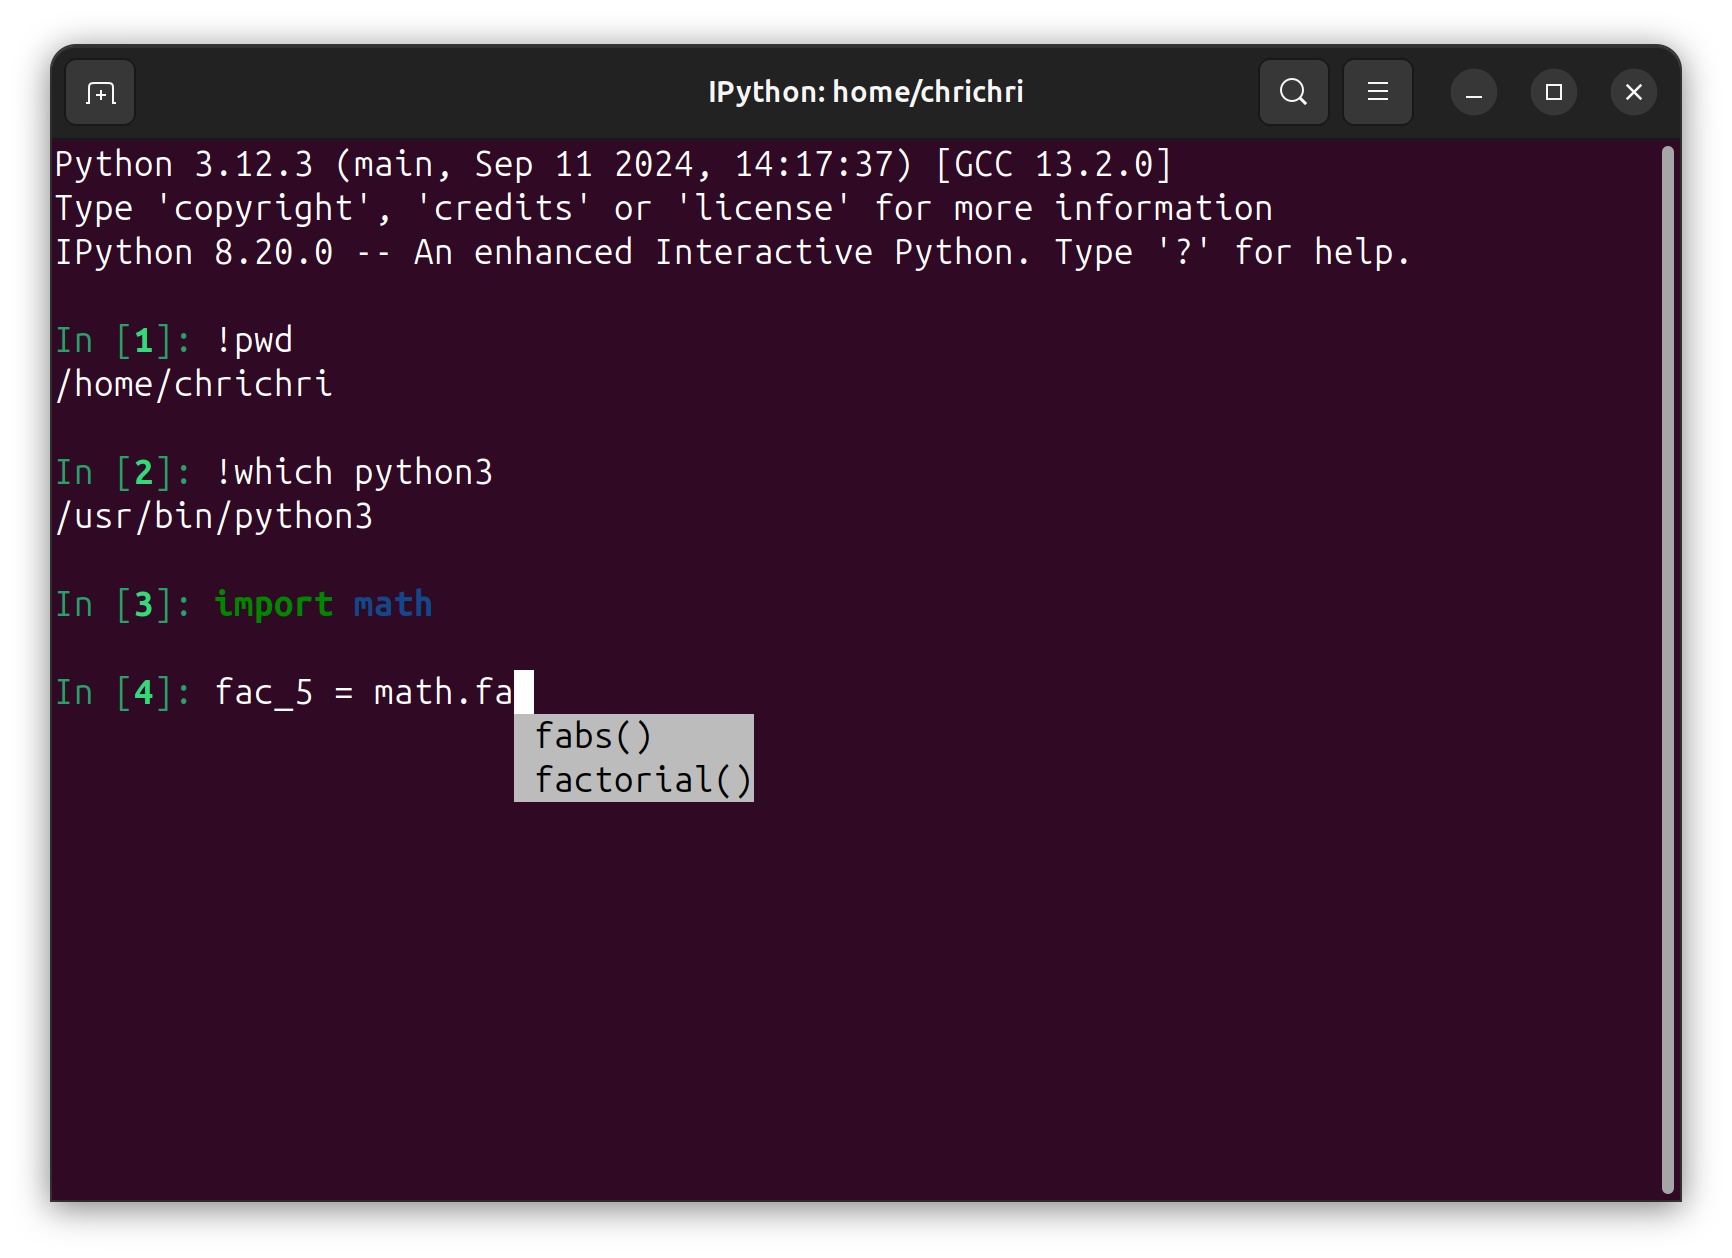
\includegraphics[width=8cm]{image/repl}
        \end{center}
        S'il est installé sur la machine, il s'intègre automatiquement à PyCharm et devient sa \textquote{Python Console}.
    \end{frame}

    \begin{frame}{Les environnements de développement}{Le Jupyter Notebook}
        \begin{center}
            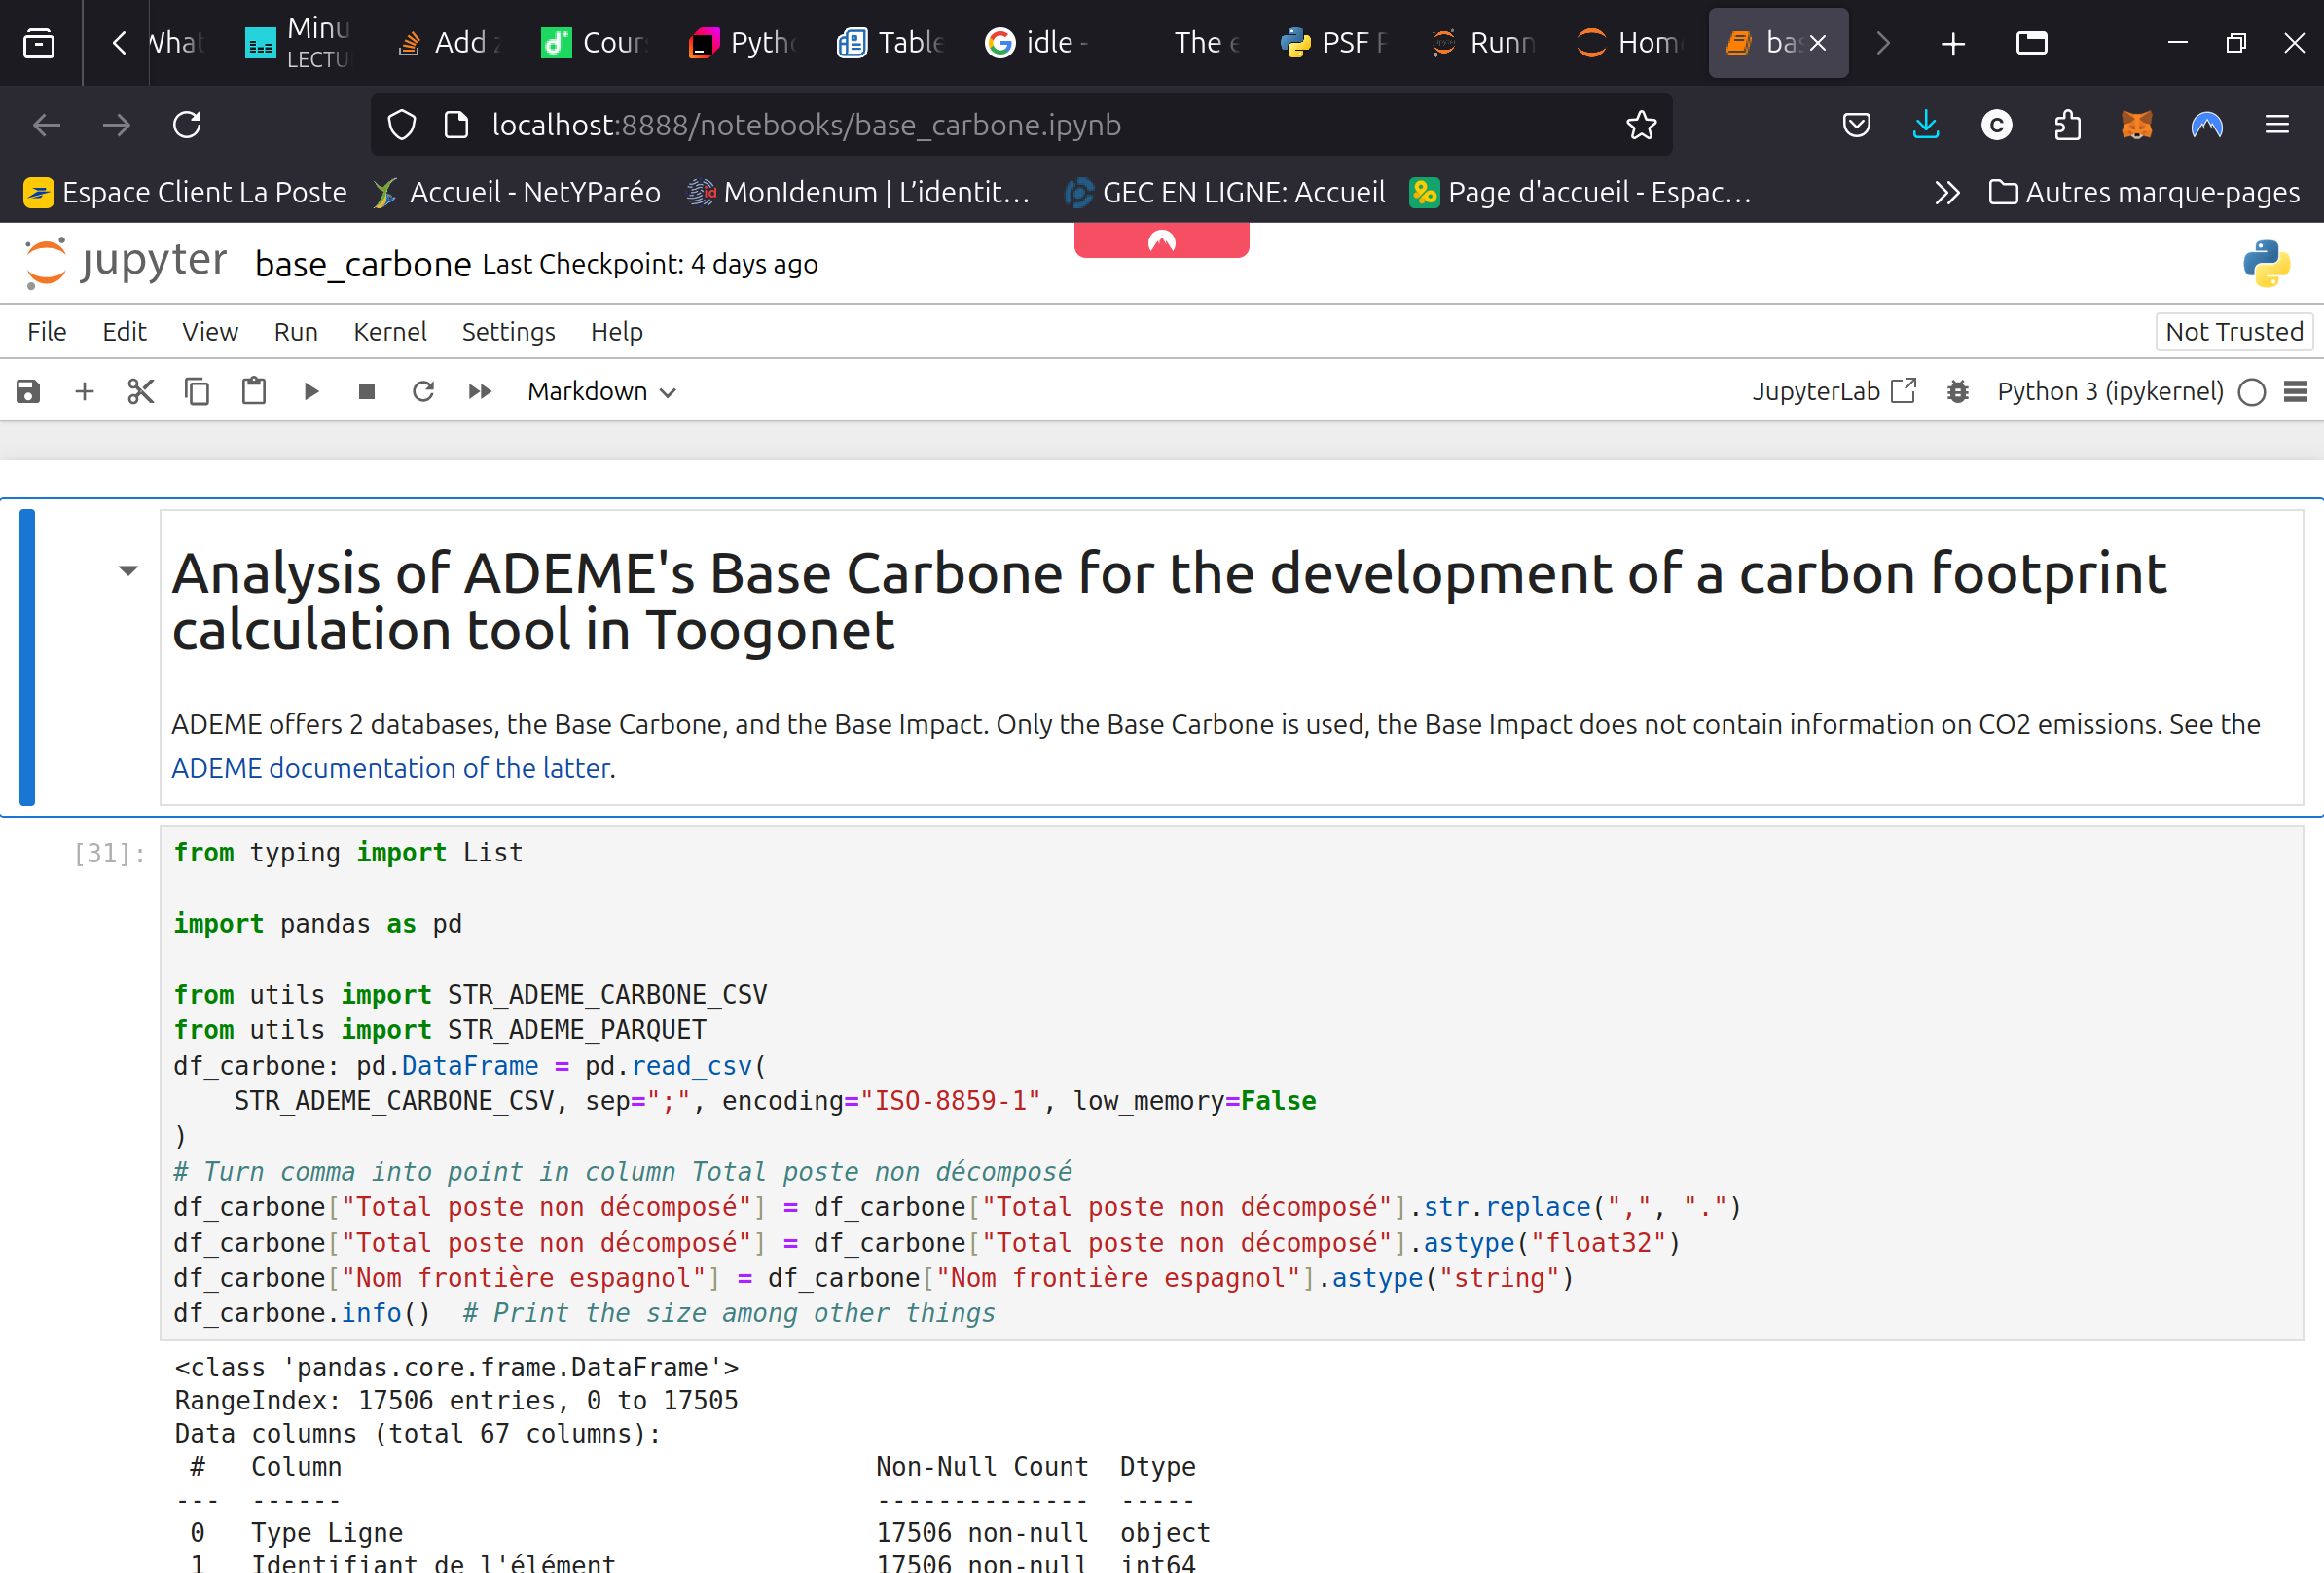
\includegraphics[width=12cm]{image/jupyter-notebook}
        \end{center}
    \end{frame}

    \begin{frame}{Les environnements de développement}{Jupyter et IPython dans PyCharm}
        \begin{center}
            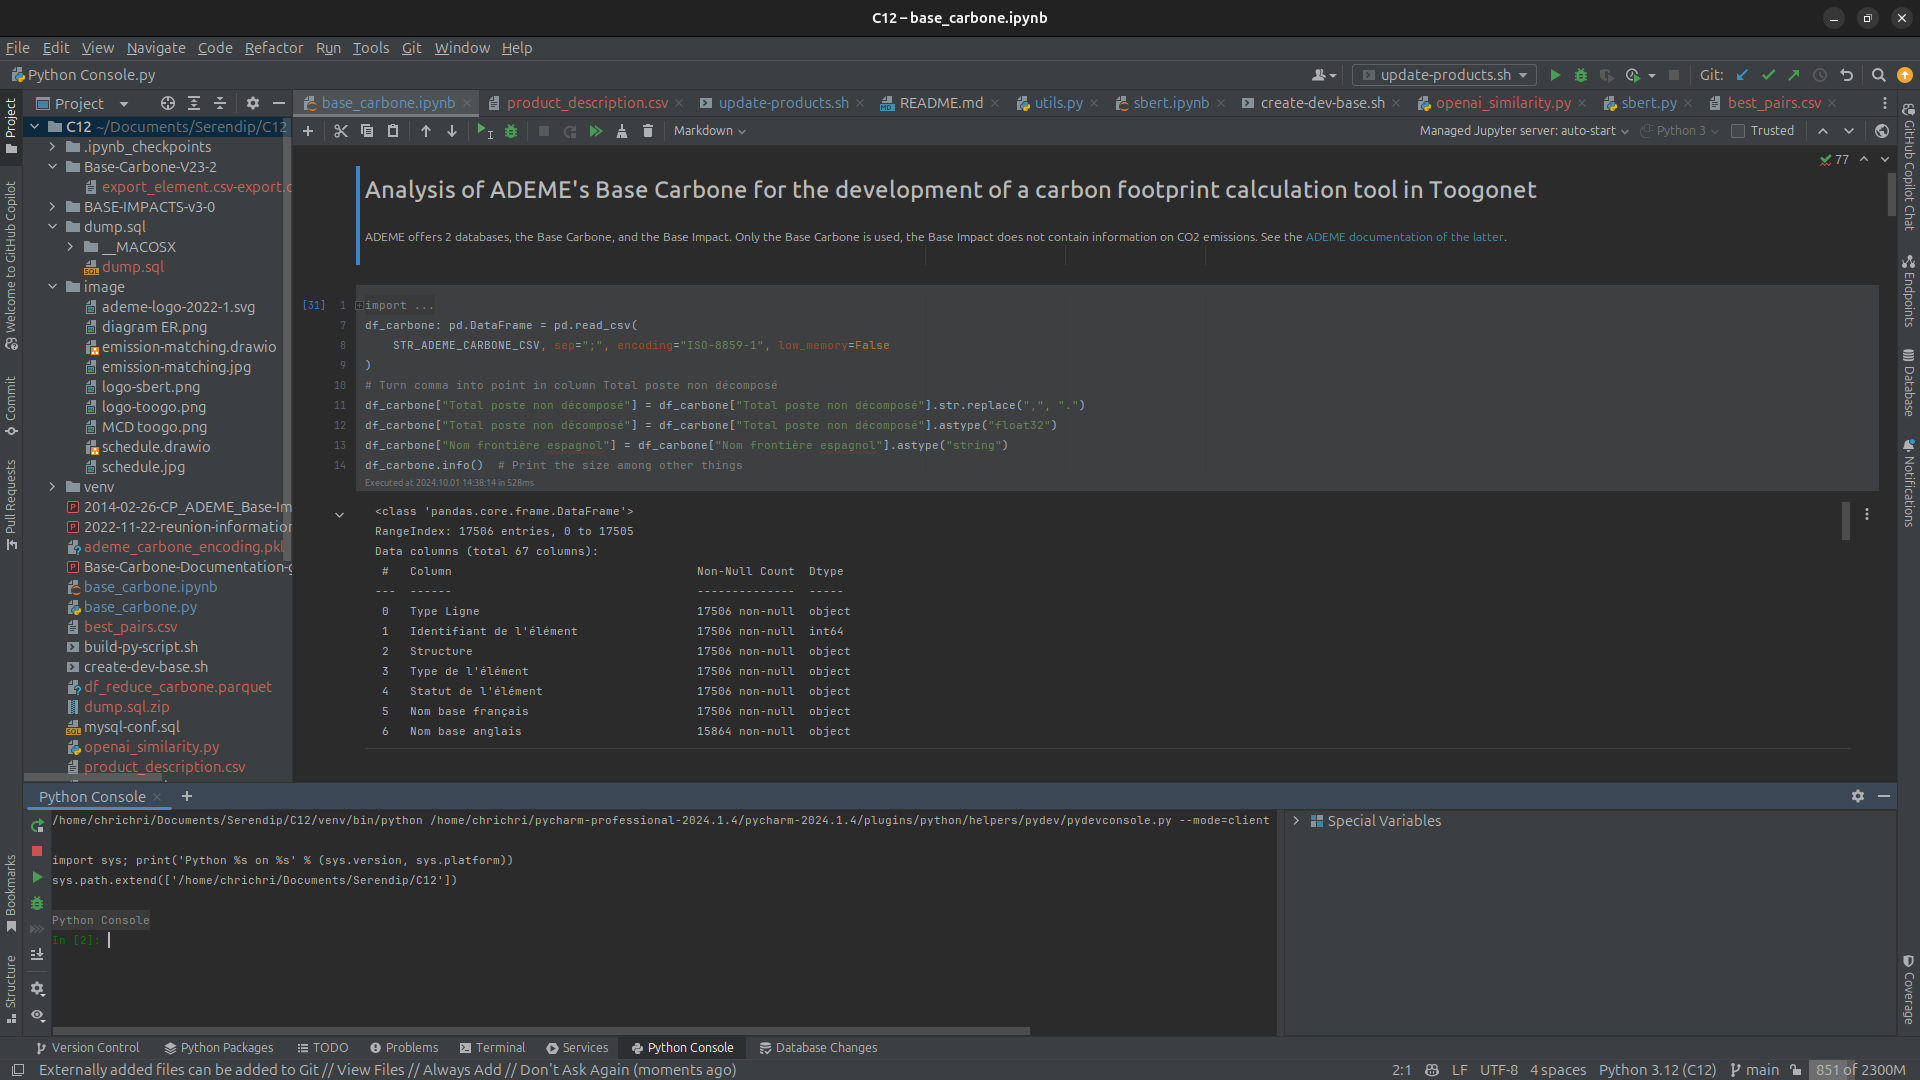
\includegraphics[width=11cm]{image/pycharm-notebook-repl}
        \end{center}
    \end{frame}

    \begin{frame}{Les environnements de développement}{Jupyter et IPython dans PyCharm}
        PyCharm est en version gratuite sur \url{https://www.jetbrains.com/pycharm/download/}, en communautaire, pour absolument tous usages~!
        \bigbreak
        IPython et Jupyter sont des packages qui s'installent à partir du gestionnaire de package de Python, \lstinline{pip}~:
        \begin{itemize}
            \item \lstinline{pip install ipython}
            \item \lstinline{pip install jupyter}, mais cette commande est à privilégier dans un virtual environnement.
            Le concept de virtual environnement sera développé dans les chapitres suivants.
        \end{itemize}
    \end{frame}


    \section{Premiers pas}\label{sec:first-steps}
    \begin{frame}{Premiers pas}{Mes premières variables et algorithme}
        Ouvrir dans Pycharm le notebook \url{https://github.com/DigicompClassesByPapIT/Python/blob/main/1_premiers_pas.ipynb}.
        \bigbreak
        Ce dernier expose des concepts de base comme~:
        \begin{itemize}
            \item Les variables
            \item Les opérateurs arithmétiques
            \item Les opérations logiques
            \item Les commentaires
            \item Les types de base
        \end{itemize}
    \end{frame}


    \section{Licence CC}\label{sec:licence}

    \begin{frame}{Licence}{Licence Creative Commons}
        Support de cours sous licence Creative Commons BY-NC-ND~.
        \bigbreak
        Vous pouvez donc, partager, copier, distribuer le document.
        \bigbreak
        Attribution requise à PapIT SASU - Pas d’utilisation commerciale - Pas de modification
        \bigbreak
        \centering
        
\includegraphics[width=5cm]{image/by-nc-nd-logo}
    \end{frame}


\end{document}
